\section{Introduction}

Evolutionary computation (EC) researchers devote substantial attention to understanding how to promote coexistence between lineages % @CAO should this be "subpopulations" rather than "lineages"?
%@ELD: interesting question. I think subpopulations implies some sort of artificial division. Is your objection to "lineages" that technically the entire population comes from a single lineage?
%@CAO: Prospectively, the entire population comes from a single lineage; retrospectively, a lineage is a single line-of-descent.  I'd often jump to the word clade here, but that would imply asexual population.  I'm okay with just leaving lineages for now.
exploring different regions of a fitness landscape~\cite{goldberg_genetic_1987,mahfoud_niching_1995, mouret_using_2009,pugh_confronting_2015}. 
Promoting diversity in an evolving population is important for EC because it reduces premature convergence on suboptimal fitness peaks while still encouraging both exploration and exploitation. However, some types of diversity facilitate finding global optima better than other types. For example, a high mutation rate generates more new genotypes, but this increased exploration sacrifices exploitation of promising prospective solutions; the population plows ahead exploring rather than refining the solutions found.

Even amongst more advanced diversity-promoting approaches, some produce forms of diversity that are spread across the fitness landscape in ways that appear to be more or less conducive to solving a given problem (see, for example, the difference between the probe and behavioral methods in~\cite{mouret_using_2009}, or the different evolutionary potential observed at equivalent diversity levels in~\cite{walker_evolutionary_2012}). Although, we have a high-level idea of why many techniques promote diversity, the mechanistic details by which these populations spread across the fitness landscape are less well understood.
For example, fitness sharing~\cite{goldberg_genetic_1987} promotes diversity via negative density dependence. Does this diversity represent qualitatively different portions of the fitness landscape than, for instance, lexicase selection~\cite{spector_assessment_2012}?
%The answer to this question depends on subtle differences in the evolutionary pressures that these different selection schemes place on the evolving population, which we are working to untangle.

Because techniques for promoting diversity rely on creating interactions between individuals in the population (beyond basic competition for space in the next generation), they are, by definition, creating simple ecologies. Ecologists have developed rigorous theory to predict how ecological communities change over time and are exploring their effects on evolutionary dynamics.
A particularly popular area of study is the conditions under which long-term stable coexistence between different species is possible~\cite{pacala_limiting_1994, chesson_mechanisms_2000,chase_ecological_2003,letten_linking_2017}. Predicting stable coexistence in EC populations allows us to determine which types of pathways through a fitness landscape a given system is able to simultaneously traverse. %, a critical component of predicting which approach will be most effective in a given scenario.
This insight should apply both to choosing an appropriate diversity maintenance technique and to setting its parameters.
Additionally, an improved mechanistic understanding of why existing algorithms work should facilitate building more effective variations of those algorithms.

There are two main sets of tools from ecology that we expect can be helpful for analyzing evolving EC communities: mathematical theory and empirical measurements.
Ecologists use mathematical theory to make \textit{a priori} predictions about the fate of natural communities.  However, translating these predictions to work with EC systems requires careful attention to implicit assumptions about nature that may or may not carry over. For instance, ecologists can safely assume that organisms inhabit a three-dimensional Euclidean space.
A more substantial problem is that most ecological theory assumes that
evolution is too slow
to be relevant and attempting to introduce evolution can create messy feedback loops (although eco-evolutionary dynamics research has begun to bridge this gap).
Another important limitation is that equations in ecology generally calculate the average or expected behavior of a system. Such results can be misleading in highly contingent processes, such as evolution.
%@CAO: Perhaps "contingent" rather than "stochastic" in the sentence above?  I think what we're trying to get at is that one random even can dramatically change the overall outcome.  Ecology also works on stochastic effects, but like thermodynamics, there are so many of them that examining the average effects gets you the right answer.
%@ELD: Agreed. I assume people at GECCO will know what contingent means?
%@CAO: Probably?  Another option is to extend it to "in highly contingent processes where rare mutations can redirect a population into a new region of the fitness landscape with different properties."
%@ELD: I like that, but it's so long...
%@CAO: Okay, let's keep this note here and we'll see how much room we have in the end (ha!)
Nonetheless, mathematical theory is a useful starting point for predictions. As such, we will lay some groundwork here for using it to guide development of EC systems.

Empirical measurements complement mathematical theory, allowing researchers to assess predictions and refine theoretical frameworks. 
Furthermore, empirical measurements allow us to uncover general patterns even in situations where theory is lacking. 
%For example, 
To this end, ecologists have developed a toolbox of techniques to evaluate the diversity of a community.
%ELD: My one objection to adding "For example" is that this isn't just an example, it's the main point of the paper
%@CAO: Agreed!
Some of these metrics, such as richness (number of unique species) and Shannon diversity (entropy) are already used
in EC.
Other valuable metrics have not yet been adopted in EC. Phylogenetic diversity~\cite{winter_phylogenetic_2013}, for example, can assess the extent to which an algorithm is maintaining independent subpopulations exploring distinct regions of the fitness landscape vs. organisms that only recently diverged from a common ancestor,
a distinction that impacts how useful the population diversity is likely to be. We can also use empirical ecological measurements to assess hypothesized mechanisms
for different diversity maintenance techniques.
For example, ecologists often build graphs representing the pairwise interactions between community members; the topology of these graphs
signals how the community is likely to change over time~\cite{fontaine_ecological_2011}. We can do the same for interacting communities in EC.

% @CAO: This next paragraph can be useful, but given our space limitations, I think we should cut it.
%@ELD: Alex and Matthew thought it was a pretty abrupt transition without it, but I've also cleaned up the next section since then
% In the rest of this section, we will provide a little bit more background on ecological theory and the selection schemes that we'll be exploring with it. In the rest of this paper, we will explore what this framework can tell us about evolutionary computation and lay the groundwork for easier application of ecological ideas to evolutionary computation in the future.

\subsection{Ecological theory}

One way that ecological theory can inform EC is to identify conditions under which different types of organisms can or cannot coexist. The ability to predict coexistence dynamics will inform us about types of lineages that can simultaneously explore the fitness landscape. As such, determining coexistence criteria is a primary focus of this paper. %Conveniently, this issue is also of central importance to ecologists.

Initial work on coexistence in ecology focused on competition for resources that are both \textit{limited} in quantity and \textit{limiting}
% in the sense that they determine
of the growth rate of species relying on them. The most important value for determining coexistence in this context is a species' $R^{*}$, the resource availability level at which the species' growth rate is 0. In the simplest case, where species are competing for a single resource, the species with the lowest $R^*$ 
should out-compete the others~\cite{grover_resource_1997}. That species' population will continue to increase, depleting the resource until it reaches the species' $R^*$; meanwhile, the resource availability will dip below the other species' $R^*$, causing their populations to decrease. Adding additional resource types introduces the potential for stable coexistence among multiple species if each species is a better competitor for a different resource and consumes more of that resource~\cite{chase_ecological_2003} (summarized in~\cite{letten_linking_2017}). Note that we use the word ``species'' here to be consistent with ecology; the same insights apply to other taxonomic units, such as phenotypes, genotypes, and individuals. In most cases, these are more appropriate taxonomic units in the context of EC.

This resource-mediated coexistence effect is an instance of a broader rule: species can coexist if individuals of each species compete with each other more than they compete with individuals of other species~\cite{chesson_mechanisms_2000}. This rule works because it forces species to be self-limiting, creating negative frequency dependent dynamics where each additional member of a species reduces that species' growth rate~\cite{adler_niche_2007}. The magnitude of difference between interspecific (between species) and intraspecific (within species) competition that is required to enable long-term stable coexistence is determined by the difference in the fitness of the two species. If one species is dramatically more fit, it can drive the other to extinction even with limited competition~\cite{chesson_mechanisms_2000}. Ecologists draw a distinction between ``stabilizing'' dynamics, which alter the ratio of interspecific competition and intraspecific competition, and ``equalizing'' dynamics which alter the difference in fitness between two species~\cite{adler_niche_2007}. In the absence of any stabilizing dynamics, equalizing dynamics lead to an unstable equilibrium; even if two species have identical fitness, one should eventually drift to extinction. Stabilizing dynamics, on the other hand, actively correct any deviation from equilibrium.
%populations of each species.
%@CAO: I think the rest of this paragraph makes an important point, but it's not critical to the overall message of the paper.  If we need to cut more, this might be a good spot.
%@ELD: See what you think after reading section 2, but you're probably right
%@CAO: I kept the first couple of sentences (which I agree become relevant!) and deleted the rest.
Note that in biology, ``fitness'' refers strictly to reproductive output. This definition is in contrast to the externally-defined ``fitness functions'' used in EC to determine competitive advantage.
%Thus, approaches such as Hierarchical Fair Competition~\cite{hu_hierarchical_2005} and Age-Layered Population Structures~\cite{hornby_alps:_2006}, which give additional offspring to low-fitness individuals without adjusting their fitness as defined by the fitness function, would be examples of equalizing dynamics.

If we consider more heterogeneous environments, there is another mechanism for species coexistence: spatial segregation due to different environmental conditions. For example, one region might require tolerance to extreme heat, while another might require tolerance to acidic soil. In this case, species would only compete when both could inhabit the same regions.

What do these coexistence dynamics mean for EC? First, when choosing parameters, we should consider the circumstances under which they promote coexistence.  When two independent lineages are traversing the fitness landscape, what genotypic or phenotypic differences are required for them to both stably persist?
Second, when designing selection schemes, we should determine how many lineages we want to co-exist and how frequently we want lineages to turn over.  If it is costly to stochastically lose established lineages, we should consider including stabilizing dynamics in addition to or in place of equalizing dynamics. 
Finally, we should give careful thought to the metaphors that we use to compare EC to biological populations; determining whether a given selection scheme is more akin to competition for resources, spatially segregated habitats, or something else all-together will make it much easier to draw parallels. If we can show that a system in EC is isomorphic to a system in biology, we can rapidly import insights from biological research into how that system behaves.
%@CAO: I feel like it might be worth noting that there are MANY more biologists than there are evolutionary computation folks, but I couldn't figure out how to say that succinctly without it also looking awkward.
%@ELD: that might be a worthwhile point to make in the conclusions

\subsection{Empirical ecological techniques}

Empirical ecologists seek to find general patterns in complex, messy data. While data from EC may be less noisy than field data, the interconnections within any ecological community are still complex. % and messy.
%@CAO: Note change in above sentence and make sure you agree.
%@ELD: I'm a little unsure about "messy" - things like standard Lotka-Volterra dynamics aren't that messy, and if you look really hard you can find ecosystems where that's most of what's happening. I guess that calls "complex" into question too...
Ecologists have developed many tools for extracting meaning from this complexity, which may be equally helpful in trying to understand the fine-scale dynamics of EC systems. Here we focus on two approaches: phylogenetic analysis and interaction networks.

\subsubsection{Phylogenetic analysis}
Phylogenetic analysis refers to a suite of metrics that are used to summarize the topology of a populations' phylogeny (ancestry tree)~\cite{winter_phylogenetic_2013}. In biology, these trees generally need to be inferred from extant species, but in EC we can record the actual tree as it forms.
Many of these methods measure the amount of evolutionary history discernible in a population. For example, evolving sub-populations that have stably coexisted for a long time will reflect deeper evolutionary history than a single population that is all descended from a recent common ancestor. Even if the latter population contains many unique phenotypes, they will all be relatively close to each other on the fitness landscape. As such, the population is likely exploring only one basin of attraction within the fitness landscape at a time, limiting the rate of adaptation.
%@CAO: Can we assume they know what a basin of attraction is?  Should we just call it a "primary fitness peak" or something along those lines?
%@ELD: I wonder that every time I use the phrase "basin of attraction." I tend to think it's an intuitive concept, and I see others using it without explaining it, but it's probably not ideal to assume that. That said, I feel like "primary fitness peak" loses the idea that it's not just the peak, but everything that leads there (I'd be tempted to make a watershed analogy if I thought people at GECCO were particularly likely to know what a watershed is)
Phylogenetic diversity provides more direct evidence about the efficacy of diversity maintenance techniques than the more commonly used measures of genotypic and phenotypic diversity.

Techniques for analyzing the topology of phylogenies can be split into three categories: richness (total quantity of evolutionary history represented), divergence (how spread out the population is in phylogenetic space), and regularity (how evenly is the population divided across evolutionary space)~\cite{tucker_guide_2017}. Here, we focus on richness and divergence, as our goal is to analyze selection schemes, which regularity does not offer clear insight into. %However, regularity may offer useful insights into the topology of the fitness landscape. 
A number of metrics measure phylogenetic richness and phylogenetic divergence (summarized in~\cite{winter_phylogenetic_2013} and~\cite{tucker_guide_2017}). Here, we measure phylogenetic richness with the original phylogenetic diversity metric (simply referred to as ``phylogenetic diversity'')~\cite{faith_conservation_1992}, which sums the lengths of the shortest path from each extant genotype to the most recent common ancestor.
%@CAO: I assume the use of "shortest path" here is because the metric applies to most recent common ancestors?
%@CAO: Also, we could define the abbreviation MRCA here, but I worry that too many acronyms will confuse readers.
%@ELD: It does apply to the most recent common ancestor, but "shortest path" is more to specify that you can't just take some convoluted path through the phylogeny and inflate the metric (probably more relevant in sexual populations)
%@ELD: we probably don't refer to the MRCA often enough for it to be necessary
We measure divergence as the mean pairwise distance between genotypes in the population~\cite{webb_exploring_2000}.  

Note that in most cases biologists implicitly assume that trees are rooted at the most recent common ancestor of all taxonomic units being compared. This assumption is unavoidable in the context of biology, because phylogeny reconstruction techniques cannot make inferences about anything preceding the most recent common ancestor. In EC, we have the full history. However, including it would not add additional information; phylogenetic diversity would increase by a constant for each member of the population and mean pairwise distance would not change. Note that we calculate these metrics on a per-genotype basis, 
%@CAO: Do you think we need to clarify that a genotype is a set of organisms with identical genomes?
%@ELD: maybe if we've got space...
but they can be calculated per-individual or per-phenotype.

\subsubsection{Interaction networks}
Since ecological communities are collections of interacting organisms, drawing a graph representing the network of pairwise interactions is a useful technique for understanding them~\cite{fontaine_ecological_2011}. The topology of this graph illustrates the selective pressures that organisms place on each other. Ecologists often generate these networks from knowledge of the species involved such as the fact that two species use the same limited resource and thus must compete with each other. 
Of course, in EC we can directly measure the fitness of each member of the population with and without each other member present to identify interactions.

\subsection{Selection schemes}

For the purposes of this paper, we have chosen a subset of selection schemes from the vast range of diversity maintenance techniques: fitness sharing~\cite{goldberg_genetic_1987}, lexicase selection~\cite{spector_assessment_2012}, and Eco-EA~\cite{goings_ecological_2009}. We compare these to each other, and to standard tournament selection, as a control. Specifically, we have selected a set of approaches that clearly map onto ecology. In the future, we plan to expand this framework to include a wider variety of diversity maintenance techniques. All of the selection schemes summarized below share common parameters such as population size and mutation functions.  Here we identify parameters unique to each system.
%In the remainder of this paper, we explore the ecological communities generated by these approaches. For those unfamiliar with the selection schemes we have chosen, we offer a capsule summary of each.

\subsubsection{Tournament selection}
As tournament selection does not create an ecology, we use it
as a control. Tournament selection has one distinct parameter, $T$, the number of individuals to randomly pick from the population (with replacement) for each tournament.  The fittest individual in the tournament is chosen to reproduce.
%@ELD: So it's okay to not explain what tournament selection actually is?
%@CAO: I think most people know, but the above does give a brief summary...

\subsubsection{Fitness sharing}

Fitness sharing was an early use of ecology to promote diversity in EC~\cite{goldberg_genetic_1987}. In fitness sharing, the fitness of every member of the population is reduced in proportion to the number of similar individuals (i.e. they ``share'' their fitness). Specifically, the number of other occupants of a niche is calculated by summing the sharing equation, $sh(d)$, over the population:

\begin{equation} sh(d) =    \begin{cases}
      1 - (\frac{d}{\sigma_{\text{share}}})^{\alpha} & d < \sigma_{\text{share}}\\
      0 &  d \geq \sigma_{\text{share}}  
   \end{cases}
\label{eq:fit_share}
\end{equation}
where $d$ is the distance (defined in terms of genotype or phenotype) between the individual that is currently having its fitness calculated and another member of the population, and $\alpha$ is a parameter determining the shape of the sharing function. Each individual's fitness is then divided by the sum of the sharing equation.

\subsubsection{Lexicase selection}

In lexicase selection, solutions are evaluated on a large number of criteria~\cite{spector_assessment_2012}. Traditionally, these criteria are each individual test cases, but other types of fitness functions are also effective~\cite{dolson_applying_2018}. To select an individual
to reproduce, the selection criteria are randomly reordered and the entire population is evaluated on each criterion. Only the individuals that perform best on a criterion are evaluated on the next, until only one individual remains. In case of a perfect tie, the winner is selected randomly from the remaining options.

Lexicase selection is highly effective at solving challenging problems in genetic programming~\cite{helmuth_general_2015,helmuth_solving_2015} while maintaining diverse populations~\cite{helmuth_effects_2016}. Prior work on the population dynamics of lexicase selection has noted the surprising prevalence of ``hyperselection events,'' occasions in which a single individual is selected as a parent for the vast majority of the next generation~\cite{mcphee_using_2016}. Given lexicase selection's success at maintaining diversity, the fact that such events occurred at all was unexpected. Further research, however, has suggested that these events are not important to lexicase selection's success at solving challenging problems and maintaining diversity~\cite{helmuth_impact_2016}.
%@CAO: Should we say more about this?  Why aren't they important?  Do they hinder problem solving?  Should they be stopped?  Not that I think we should take more room on this here; if anything we want to spare only another line or so.
%@ELD: The paper doesn't really figure out why they don't matter, just that they don't (it made them impossible and found that the overall outcome didn't really change)
Additional case studies of phylogenetic trees generated by lexicase selection
suggest that lexicase selection promotes the existence of
%found
%@ELD: Found is kind of a strong word for their results...
sub-populations that are focused on a specific selection criterion~\cite{mcphee_visualizing_2016}.

%\subsubsection{%MAP-Elites}

%In MAP-Elites~\cite{mouret_illuminating_2015}, the user selects some number of dimensions along which they would like to see a diversity of solutions, and the search space defined by those dimensions is discretized into bins. Whenever a new individual is created, it is assessed on each dimension and put into the corresponding bin is located. If the bin is empty, or the individual currently occupying it has lower fitness than the newcomer, the newly created individual is placed into the bin, replacing any existing occupant. If the bin is already occupied by an individual with higher fitness than the new individual, the new individual is discarded. Not only has this approach proven effective at solving problems, particularly those where a variety of phenotypic options are desirable~\cite{cully_robots_2015}, it also provides insight intro trade-offs inherent in the search space.

\subsubsection{Eco-EA}

Eco-EA is an approach to solving complex problems by associating limited resources with simpler problems~\cite{goings_ecological_2009,goings_natural_2010,goings_ecology-based_2012}. These simpler problems can be components of the larger problem, test cases, or other related tasks that may form building blocks for a global solution. Resources accumulate until a solution to the corresponding sub-problem is discovered. When a population first solves a sub-problem, the associated resource is plentiful, dramatically boosting the fitness of individuals that use it.
As the number of individuals using the resource increases, it become less valuable. As long as there is a cost to attempting to use each resource, negative frequency dependence fosters small, but stable sub-populations associated with each resource. 
%However, full negative frequency dependence is only possible if there is a cost to attempting to use a resource. Without a cost, the benefit of using a resource diminishes as the number of individuals using it increases, but there is never pressure \textit{not} to use it. As a result, without a cost, there is no pressure to maintain diversity. Early work with Eco-EA featured problems with inherent tradeoffs, creating an implicit cost \cite{goings_ecological_2009,goings_ecology-based_2012}. When Eco-EA was extended to other
For
problems without such tradeoffs, an explicit cost is introduced~\cite{dolson_applying_2018}.
%@CAO: I don't think we need to go into the gory details about figuring out the need for a cost.
%@ELD: Since they're about the subtlelties of negative frequency dependence, they seemed relatively on topic for this paper, but I'm fine with removing them. Leaving this here in case we have extra space.
%Eco-EA has proven to be effective at evolving diverse 

\section{Ecology in EC systems}

In this section, we discuss how each of our chosen EC selection schemes can be intuitively mapped onto ecology. We believe that these metaphors will facilitate a two-way flow of ideas between fields. With the aid of these metaphors, we consider how to calculate two ecologically-important factors: the probability of an individual being selected to have an offspring (i.e. biological fitness, $W$) and the conditions under which stable coexistence is possible. The former is critical for calculating interaction networks within ecological communities (see Section 3.1) and the latter provides insight into not only the amount of diversity that a selection scheme promotes, but how the population is situated across the fitness landscape.

\subsection{Tournament selection}
Individuals in tournament selection have no interaction beyond competition for space in the next population. Since this competition
affects all individuals equally, tournament selection approximates a condition where there is no ecological interaction. Nature lacks comparable situations, as ecology is nearly ubiquitous outside of carefully controlled experimental environments (although evolutionary theorists often make this simplifying assumption).
%@CAO: Would it be reasonable to tack on to the previous sentence ", although evolutionary theorists often make this simplifying assumption."
%@ELD: I think so.
%@ELD: Actually that makes for kind of an awkward sentence. I think it's better as a parenthetical?
The absence of ecology in tournament selection means that stable coexistence is impossible in the long term. 

Calculating the biological fitness, $W$, of an individual in tournament selection requires determining the proportion of the population with lower fitness score than that individual's, $p_{\text{worse}}$. Based on this number, we can calculate the probability of the focal individual winning a tournament. We must also account for ties based on $p_{\text{equal}}$, the proportion of the population with a fitness score equal to the focal individual's. For the purposes of this paper, we use a tournament size of $T=2$, making this equation:
%\begin{equation}
%W_{i} = 2\times p_{\text{worse}} \times \frac{1}{\text{population size}} + p_{\text{equal}} \times \frac{1}{\text{population size}}
%\label{tournament_equation}
%\end{equation}
\begin{equation}
W_{i} = \frac{2\times p_{\text{worse}} + p_{\text{equal}}}{\text{population size}}
\label{tournament_equation}
\end{equation}
Note that $p_{\text{worse}}$ is multiplied by two because individual $i$ could be chosen either first or second. For $p_{\text{equal}}$, the two is canceled out because each member of the tournament only has a $0.5$ chance of winning a tie.

\subsection{Fitness sharing}

Fitness sharing operates on the basic ecological assumption that individuals compete more with individuals that they are more similar to. The most intuitive ecological scenario to compare fitness sharing to is one where a population consumes a single, continuously-varying resource. In cases where the distance function is calculated over a discrete number of dimensions (e.g. Euclidean distance between two vectors of equal length), the resource can be thought of as varying over the same number of dimensions. An analogous situation in ecology is that of Darwin's finches~\cite{schluter_ecological_1985}. All of these finches eat seeds, which vary along dimensions such as size and shape. Each species of finch has a beak that is best adapted to eat seeds near a target size and shape.
Over evolutionary time, the finch species have partitioned the space of possible beak morphologies into stable niches specialized on different seed types. In the context of fitness sharing, we expect the population to partition the space of possible phenotypes into stable niches. The theory of limiting similarity suggests that these niches should be somewhat separated from each other in genotypic/phenotypic space~\cite{pacala_limiting_1994}. Fitness sharing results suggest that these niches are often associated with peaks in the fitness landscape~\cite{goldberg_genetic_1987}. 

%Fun fact - this paper by Deb was published just 1 year before Chesson's first paper showing the same result in ecology!

%ELD: Also, more general question: I feel like this is actually a pretty cool result - should I be making a bigger deal of it? For instance, I had to do a bit of algebra to get Deb's equation into this form. Should I be showing that? I'm not used to dealing with math results.
%@CAO: Interesting.  If you haven't shown this before then yes, I do agree that it's a big result.  In addition to putting it hear, you should absolutely put it in the diversity review.
%@ELD: I've certainly never shown it before, and I don't think anyone else has either. Early in the lit review for this paper I googled "'evolutionary computation' Chesson" and the only results were a paper I wrote, a paper Bess wrote, and one of Ben's students' dissertation.

Deb and Goldberg have already established the criteria for stable coexistence in fitness sharing~\cite{deb_investigation_1989}, which is mathematically identical to Chesson's predictions under modern coexistence theory~\cite{chesson_mechanisms_2000} (converted into this form in ~\cite{letten_linking_2017}):

\begin{equation}
\frac{k_1}{k_2} \leq \frac{1}{\rho}
\label{eq:share_coexist_1}
\end{equation}
where $k_1$ and $k_2$ are the fitness function scores of the fitter and less fit individual respectively and $\rho$ is the niche count between these two individuals, as calculated by Equation \ref{eq:fit_share}. We chose these symbols to be consistent with Chesson's~\cite{chesson_mechanisms_2000}. Note that in Chesson's framework, $\rho$ generalizes to be the amount of niche overlap between the two individuals. The intensity of stabilizing dynamics (i.e. negative frequency dependence) can be calculated as $1-\rho$. Equation \ref{eq:share_coexist_1} essentially states that, for stable coexistence to occur, the niche overlap must be less than 1. The smaller $\rho$ is, the greater the difference in fitness values it is capable of stabilizing.

The biological fitness, $W$, of individuals in fitness sharing can be calculated by modifying fitness scores based on Equation \ref{eq:fit_share} and then applying Equation \ref{tournament_equation} based on the adjusted scores.

\subsection{Lexicase selection}

In ecological terms, lexicase selection creates a vast number of niches nested within each other. While it is tempting to use a resource metaphor to understand the competition within these niches, the concept of resources does not clearly map onto lexicase selection. Whereas using a resource harms all other individuals that use that resource, improving on a selection criterion in lexicase selection only harms a (usually small) subset of the population. Instead, we argue that population structure is a more apt metaphor.% for lexicase selection. 

Imagine $N!$ islands of equal size, where $N$ is the number of selection criteria. Each island corresponds to a single potential ordering of selection criteria and can only be inhabited by the individuals that are best at that ordering. This arrangement is analogous to situations in nature where niches are defined exclusively by an organism's ability to survive a set of harsh abiotic conditions. Being better able to survive these conditions increases the number of offspring an individual can have. Over time, genotypes that are better at surviving in a given set of conditions competitively exclude those that are worse at surviving there. This competitive exclusion happens more rapidly in lexicase selection than it usually would in biology, but the principle is the same. 

%One weird thing about this metaphor is that all space is adjacent. I feel like I should mention this, but I'm not sure how to, because it's a confusing concept
%@CAO: It's almost worse than that since some islands are nearer each other than others, based on the first criteron, then the second, etc.
%There are parallels to be drawn to some of the lexicase phylogeny papers, but they didn't fit in nicely.

%$N!$ is the maximum number of genotypes that should be able to stably coexist in the long term within a population under lexicase selection. 

While %islands can potentially be inhabited by 
multiple genotypes
can theoretically inhabit the same island
if they are phenotypically identical,
this coexistence will be unstable due to the lack of stabilizing dynamics to increase the populations of rare genotypes
on an island.
Eventually, all but one should stochastically go extinct. Furthermore, much as an island in nature can
experience a random catastrophic event, (e.g., a volcanic eruption), the stochastic nature of lexicase selection means that in every generation there is a chance that an island will get unlucky and not be selected. The probability of such an event progressively increases as the proportion of the population living on each island ($\frac{\text{population size}}{N!}$) decreases. %Importantly,
When the total population size is %often
less than the number of islands, %meaning that
genotypes must inhabit multiple islands to survive. Thus, stable coexistence in lexicase selection depends on whether a genotype's range (i.e. the proportion of islands it can occupy)
%, including fractions of islands in the case of ties)
%@CAO: Technically the fractions of islands comment is correct, but it has too many nuances to really explain clearly.
is large enough to survive in the long term.

In lexicase selection, an individual's range is the same as its biological fitness, $W$, because its chances of reproduction are based solely on how much space it occupies. Just as species in nature face greater risk of stochastic extinction if their range (the area they inhabit) is too small, so too do genotypes in lexicase selection. The chances of an individual with fitness $W$ surviving for $G$ generations in a population of size $S$ are given by the equation:

\begin{equation}
P(\text{survival}) = (1 - (1-W)^{S})^{G}
\end{equation}
\begin{figure}
%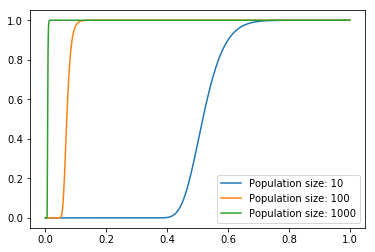
\includegraphics[width=1.5in]{figs/survival_pop_size.png}
%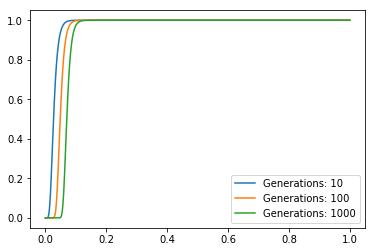
\includegraphics[width=1.5in]{figs/survival_generations.png}
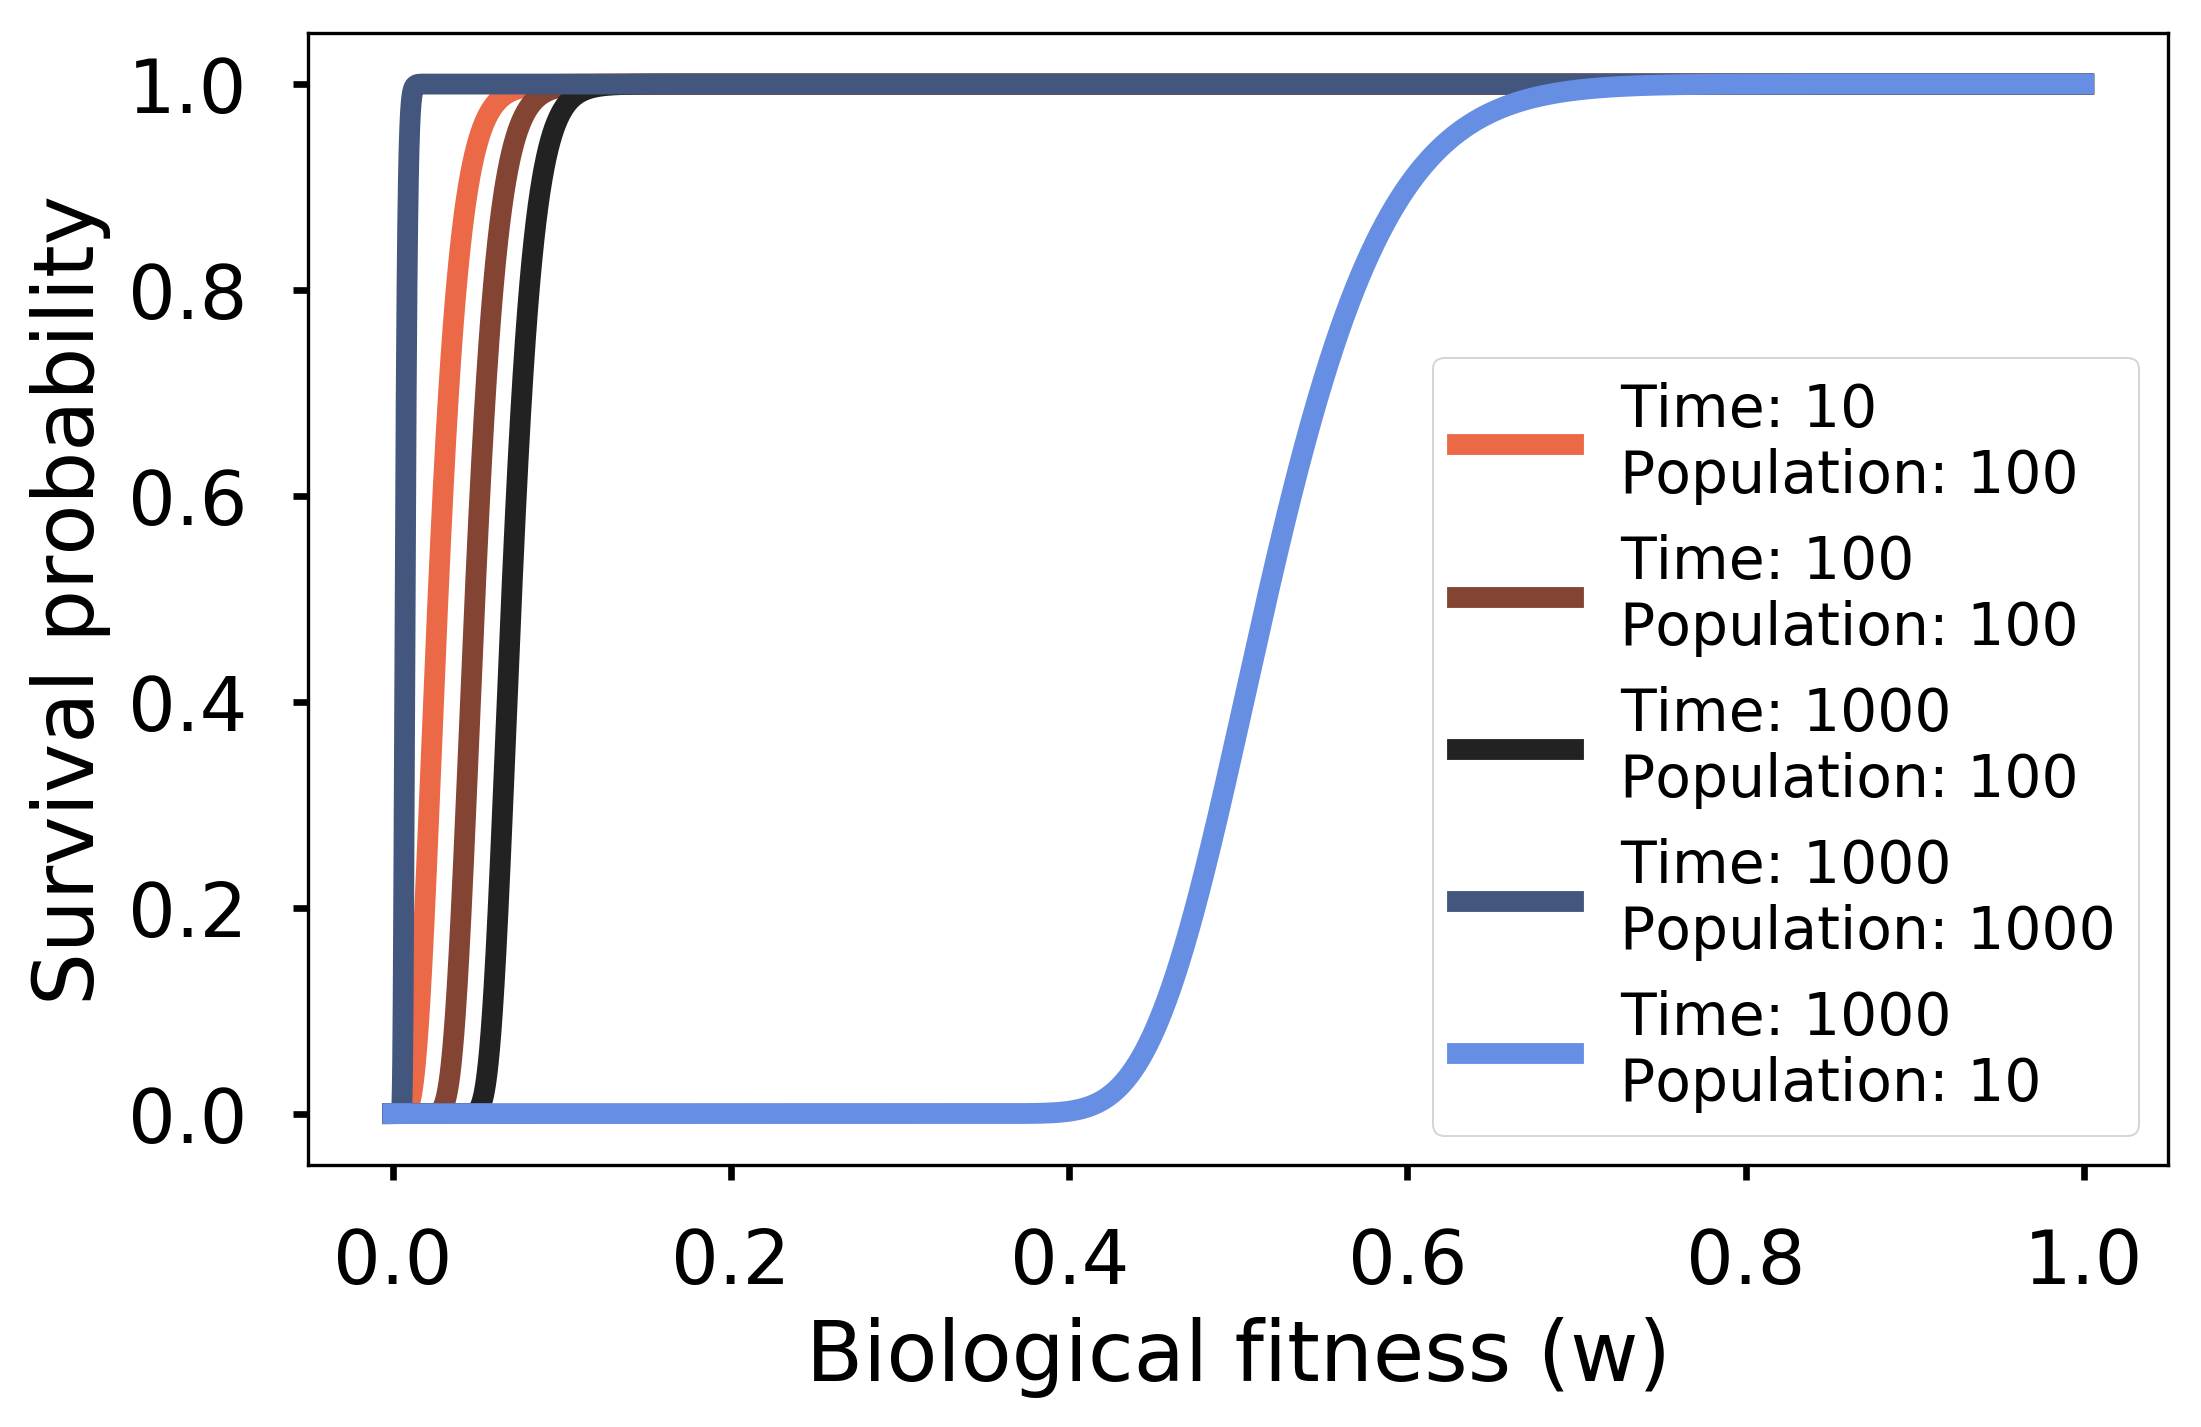
\includegraphics[width=3.4in]{figs/survival.png}
\caption{The probability of long-term survival under lexicase selection across different population sizes (S) and lengths of evolutionary time (G).}
\label{prob_survival}
\end{figure}
Plotting this function for various parameter values, we see that there is generally a cut-off where the probability of survival rises abruptly from approximately 0 to approximately 1 (see Figure \ref{prob_survival}). The value at which the transition occurs is effectively the minimal percentage of islands that a genotype must occupy in order to be expected to survive in the long term. This value is closely related to the concept of a minimum viable population in biology, and is useful to consider when making decisions about how large of a population size to use. 

%From this analysis, we can conclude that lexicase selection produces 

%The selection criteria determine which other individuals in the population a given solution is competeing with for space. 

%\subsection{MAP-Elites}

%The criteria for stable coexistence in MAP-Elites are refreshingly straightforward. Like lexicase selection, MAP-Elites can be thought of as an alternative population structure. Each location in the spatial structure can only be occupied by individuals that fall in the correct phenotypic range. Within a location, competitive exclusion happens immediately. Because each individual can only occupy one location in the population, there is no competition. All members of the population have equal biological fitness, $W$, and all are capable of stable coexistence for an infinite length of time (because individuals stay in the population until they are replaced, there isn't even a risk of stochastic extinction).

\subsection{Eco-EA}

Eco-EA is analogous to a traditional resource competition scenario in ecology. All individuals occupy the same region of space and compete with each other by targeting
the same resources. We can calculate the threshold amount of a resource in the environment needed by each individual to benefit from using it:

\begin{equation}
R^* = \frac{cost}{C_f * score}
\label{eq:ecoea-rstar}
\end{equation}
Where $cost$ is the cost of performing the corresponding task, $C_f$ is the fraction of the available resource consumed, and $score$ is how well the individual performed the task (normalized to 1). In resource competition theory terms, this value is effectively that individual's $R^*$ for that resource.\footnote{This definition is subtly different from the traditional definition of $R^*$, which states that $R^*$ is the lowest value of resource for which a species' per capita population growth is not negative~\cite{chase_ecological_2003}. We frame $R^*$ in terms of benefit rather than population growth because population growth in EC is generally restricted by competition for space in the population.} Note that a higher $score$ reduces $R^*$, meaning that the individual can benefit from the task even if less of the resource is available, making it a better competitor for that resource. Thus, as in natural ecosystems, the individual with the lowest $R^*$ can out-compete individuals with a higher $R^*$.

If a group of individuals use completely different resource types from each other, there will be a high degree of stabilization, meaning they should coexist under a wide range of fitness differences. The more complex coexistence scenario occurs when two individuals compete for the same resources. Ecologists distinguish resources that can be used interchangeably with each other (``substitutable resources'') from resources that cannot be used interchangeably (``essential resources''). Resources in Eco-EA are substitutable, because an equivalent fitness gain could be achieved using either one (up to a point); one just requires more resource to do so.  In this scenario, two individuals can stably coexist as long as they have lower $R^*$s for opposite resources, and each one consumes more of the resource it has a lower $R^*$ for. Because both $R^*$ and the amount of resource consumed are determined by the individual's score on the task associated with the resource, the latter criterion will always be met. Thus, as long as neither individual has the lowest $R^*$ for every resource, coexistence should be possible. In EC terms, this requirement boils down to each individual being Pareto dominant. As before, coexistence also requires that the individuals have somewhat similar fitnesses. The amount of stabilization (and thus the maximum fitness difference) can be calculated based on the resource consumption of each species~\cite{letten_linking_2017}.

Biological fitness, $W$, can be determined in the same way as in fitness sharing: first, calculate the adjusted fitnesses based on resource use, then use Equation \ref{tournament_equation}. 

\subsection{Summary}

As we would expect, selection schemes that successfully maintain diversity allow for long-term stable coexistence. For fitness sharing and Eco-EA, the criteria are described by Chesson's coexistence theory~\cite{chesson_mechanisms_2000}; each species/genotype/phenotype must limit itself more than it limits others (as formalized in Equation \ref{eq:share_coexist_1}). In lexicase selection, biological fitness (i.e. the proportion of ``islands'' the species dominates) must be above a cutoff described in Figure \ref{prob_survival}.

Although Eco-EA and fitness sharing have the same coexistence criteria, they have an important difference from each other: in Eco-EA, competition occurs along multiple, potentially orthogonal dimensions, whereas in fitness sharing competition is mediated through a function that summarizes all aspects of an individual. This difference should result in fewer, more intense pairwise competitive interaction in Eco-EA than in fitness sharing (although still not as few, or as intense, as those in lexicase selection). We predict that these more focused interactions will promote more useful forms of evolutionary divergence. The requirement in Eco-EA that coexisting individuals must be non-dominated suggests that individuals in Eco-EA should fall roughly along a pareto front, similarly to individuals in lexicase selection. An important distinction between these two selection schemes, however, is that lexicase selection's rigid population structure produces strong pressure for specialists, whereas generalists can be successful in Eco-EA.

\section{Empirical Methods}

%@ELD this is basically all in the intro now
%While theory offers a good mental framework to understand empirical results, it can easily get detached from reality. This issue is exacerbated in the case of systems with substantial stochasticity and feedback loops, such as evolutionary systems. In such situations, the average case predicted by theory may not actually be particularly representative. Thus, 
To confirm and extend the intuition we developed in the previous section, we now empirically investigate these selection mechanisms in the context of actual evolving populations. 

\subsection{Interaction networks}
In section 2, we predicted the competitive pressures that different selection schemes exert on populations. Here, we assess %the accuracy of 
these predictions by drawing interaction networks for real populations. % under these selection schemes. 
For simplicity, we use a population containing 10 individuals with 5 integer traits selected from a geometric distribution. Each trait represents a niche that these individuals are competing to occupy, with higher numbers corresponding to higher competitive ability. % for that niche.
For lexicase selection, each trait %position in the vector
is a selection criterion and the individual with the highest value there wins. In Eco-EA, we added a resource associated with each trait and an individual's value for that trait %at that position
defines its ability to use that resource. In fitness sharing, distance is measured as euclidean distance between sets of traits. The fitness landscape is otherwise flat. We compare the same population across all selection schemes. To calculate the effect that a given individual, $A$ has on another individual, $B$, we first calculate the fitness of $A$ in the presence of the whole population. Then we remove $B$ from the population and recalculate the fitness of $A$. The difference between these two fitnesses is the effect of $A$ on $B$. Note that these fitness values are biological fitness, i.e. the probability of being selected to reproduce, rather than the fitness produced by the fitness function.  For fitness sharing and Eco-EA, we assume a tournament size of 2 when making this calculation.

\subsection{Phylogenetic analysis of evolved populations}
What is the long-term effect of these different interaction network topologies? We arrive at a first-order approximation by analyzing the phylogenies of populations evolved under each selection scheme. Across selection schemes, the behavior of a population depends on the part of the fitness landscape that it is currently exploring. If the entire population is climbing a steep hill, all forms of diversity should be low, due to frequent selective sweeps. To asses the effect of such differences in fitness landscapes, we compare phylogenetic diversity across three different genetic programming problems believed to have qualitatively different fitness landscapes. The first task, chosen to be quickly-solvable, is calculating the square of a number. In contrast, the second task is a math problem known to be challenging: calculating numbers in the Collatz sequence~\cite{helmuth_general_2015}. The third task is the Dow chemical challenge, a real-world symbolic regression problem~\cite{white_better_2013}. We evolve linear genetic programs for 1000 generations, using 11 test cases for the squares problem and 100 test cases each for the Collatz problem and Dow chemical challenge. Phenotypes are the vectors of inverse error for each test case (so higher scores are better). Fitness is calculated as the sum of these vectors. For lexicase selection and Eco-EA, each test case corresponds to a selection criterion or resource. 

%@ELD: Do I need to go into more detail on AvidaGP?
%@CAO: Technically, yes.  Practically, there's no way we're getting that in now.  My guess is that for the final paper we'll move more text into supplemental material, and add details about AvidaGP there.

We evolved 30 populations for each selection scheme and each problem. Because of the profound effect of the sharing threshold parameter on the behavior of fitness sharing, we also performed 30 runs each of fitness sharing with five different sharing thresholds. Statistics across selection schemes were calculated using the sharing threshold with the highest phylogentic diversity. For each run, we calculated a variety of metrics, including phenotypic diversity (measured as Shannon entropy), genotypic diversity, phylogenetic diversity~\cite{faith_conservation_1992}, and mean pairwise distance of genotypes in the phylogeny~\cite{webb_exploring_2000}. Across all runs, we used a genome length of 200 and a population size of 500. We applied mutations to every new individual by randomly changing the code at up to three sites in the genome (the specific number was selected from a uniform distribution). To simplify calculation of the phylogenetic metrics, we seeded each population with a single individual that served as the common ancestor to all others.
%@ELD: It does look like this matters, but not in an easy to explain way, and it's a little off topic for the paper
For Eco-EA, we used a resource inflow rate of 100, a cost of 1, and a consumption fraction for .0025.

\subsection{Statistical methods}
That statistical significance of all comparisons of metrics across conditions was assessed using a Kruskal-Wallis test. Differences between specific conditions were assessed with a post-hoc pairwise Wilcoxon rank-sum test accompanied by a Bonferroni correction for multiple comparisons.

\subsection{Code availability}
Data for the interaction network analysis was generated using a %simple
simulation written with Python 3.6.3. Graphs were visualized using the networkx package~\cite{hagberg_exploring_2008}. The code for empirical analysis of evolved populations was written in C++ using [REMOVED FOR DOUBLE-BLIND]. Statistical analysis was performed using the R statistical computing language version 3.4.3~\cite{r_core_team_r:_2017} and graphs were made with the ggplot2 package~\cite{wickham_ggplot2:_2009}. All code for generating and analyzing the data presented in this paper is open source and available at [REMOVED FOR DOUBLE-BLIND]. 

\section{Results and Discussion}

\subsection{Interaction networks}

\begin{figure}
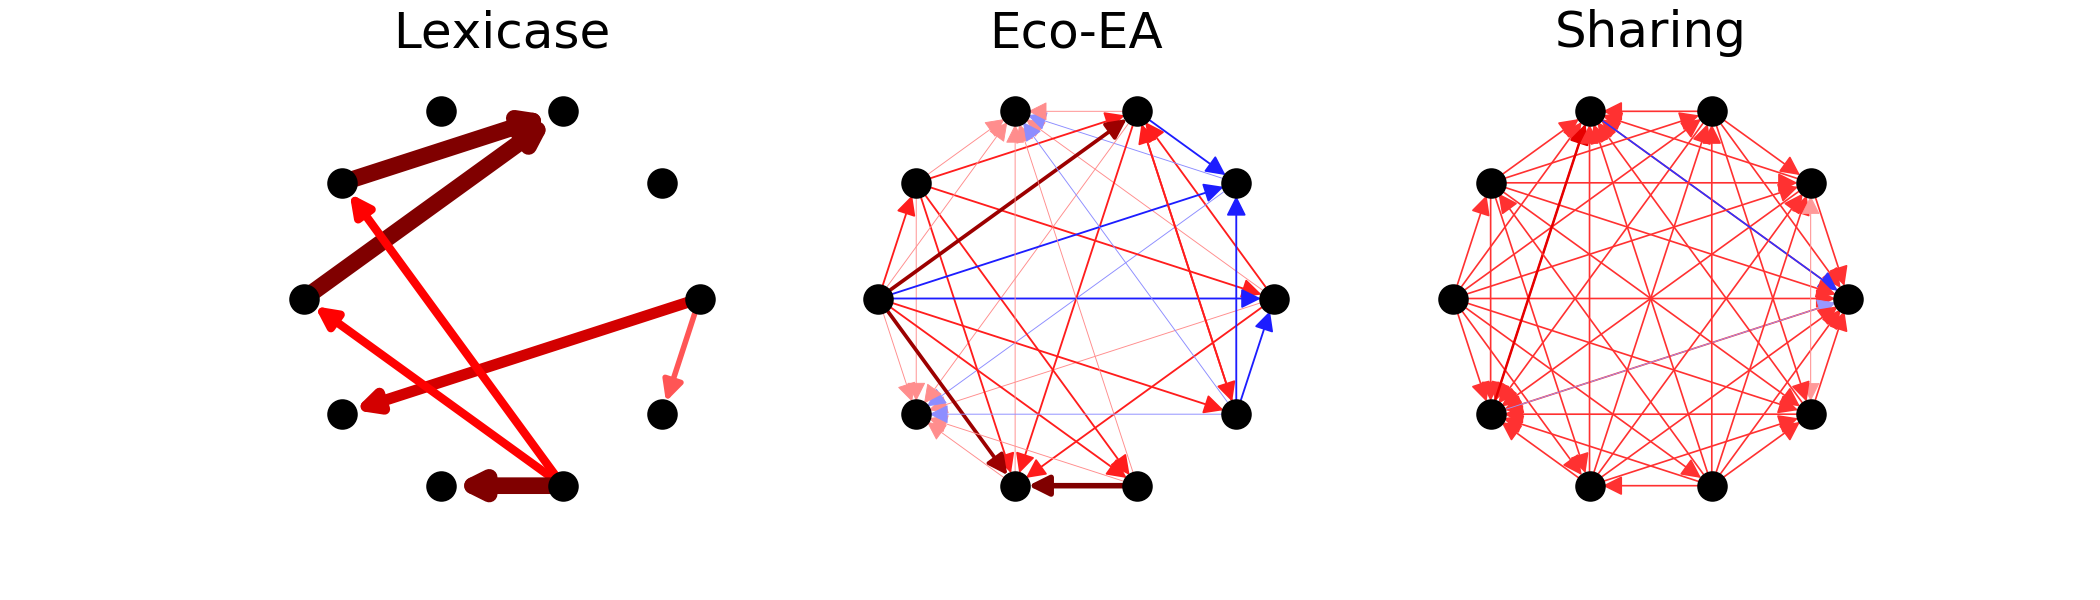
\includegraphics[width=3.5in]{figs/interaction_networks.png}
\caption{Interaction networks for the same community under three different selection schemes: lexicase selection, Eco-EA, and fitness sharing. Red edges indicate harmful interactions, blue edges indicate beneficial interactions. Edge width denotes interaction strength.}
\label{interaction_network}
\end{figure}

Different selection schemes create strikingly different interaction networks (see Figure~\ref{interaction_network}). Notably, lexicase selection's rigid population structure leads to far fewer interactions than under other schemes, and ones that are predominantly negative. Eco-EA creates far more interactions, because individuals can use different resources to different extents. Importantly, there are many beneficial interactions; if $A$ competes with $B$ and $B$ competes with $C$, $A$ can help $C$ by suppressing $B$. %Although these complex networks of interactions where once believed to produce a chaotic and unstable community~\cite{may_ecological_1973}, more recent evidence suggests that 
%@ELD: Maybe we can consider adding this back in if we have space.
These interactions imply a stabilizing dynamic between $A$ and $C$, because they indicate that $A$ is competing with $C$ less than with itself. Additionally, the Eco-EA community has many weak interactions, which can promote stabilizing dynamics community-wide~\cite{mccann_diversitystability_2000}. Lastly, in fitness sharing, most individuals harm each other approximately the same amount. The sharing threshold subtly affects interaction strength.


\subsection{Phylogenetic analysis}

\begin{figure}
%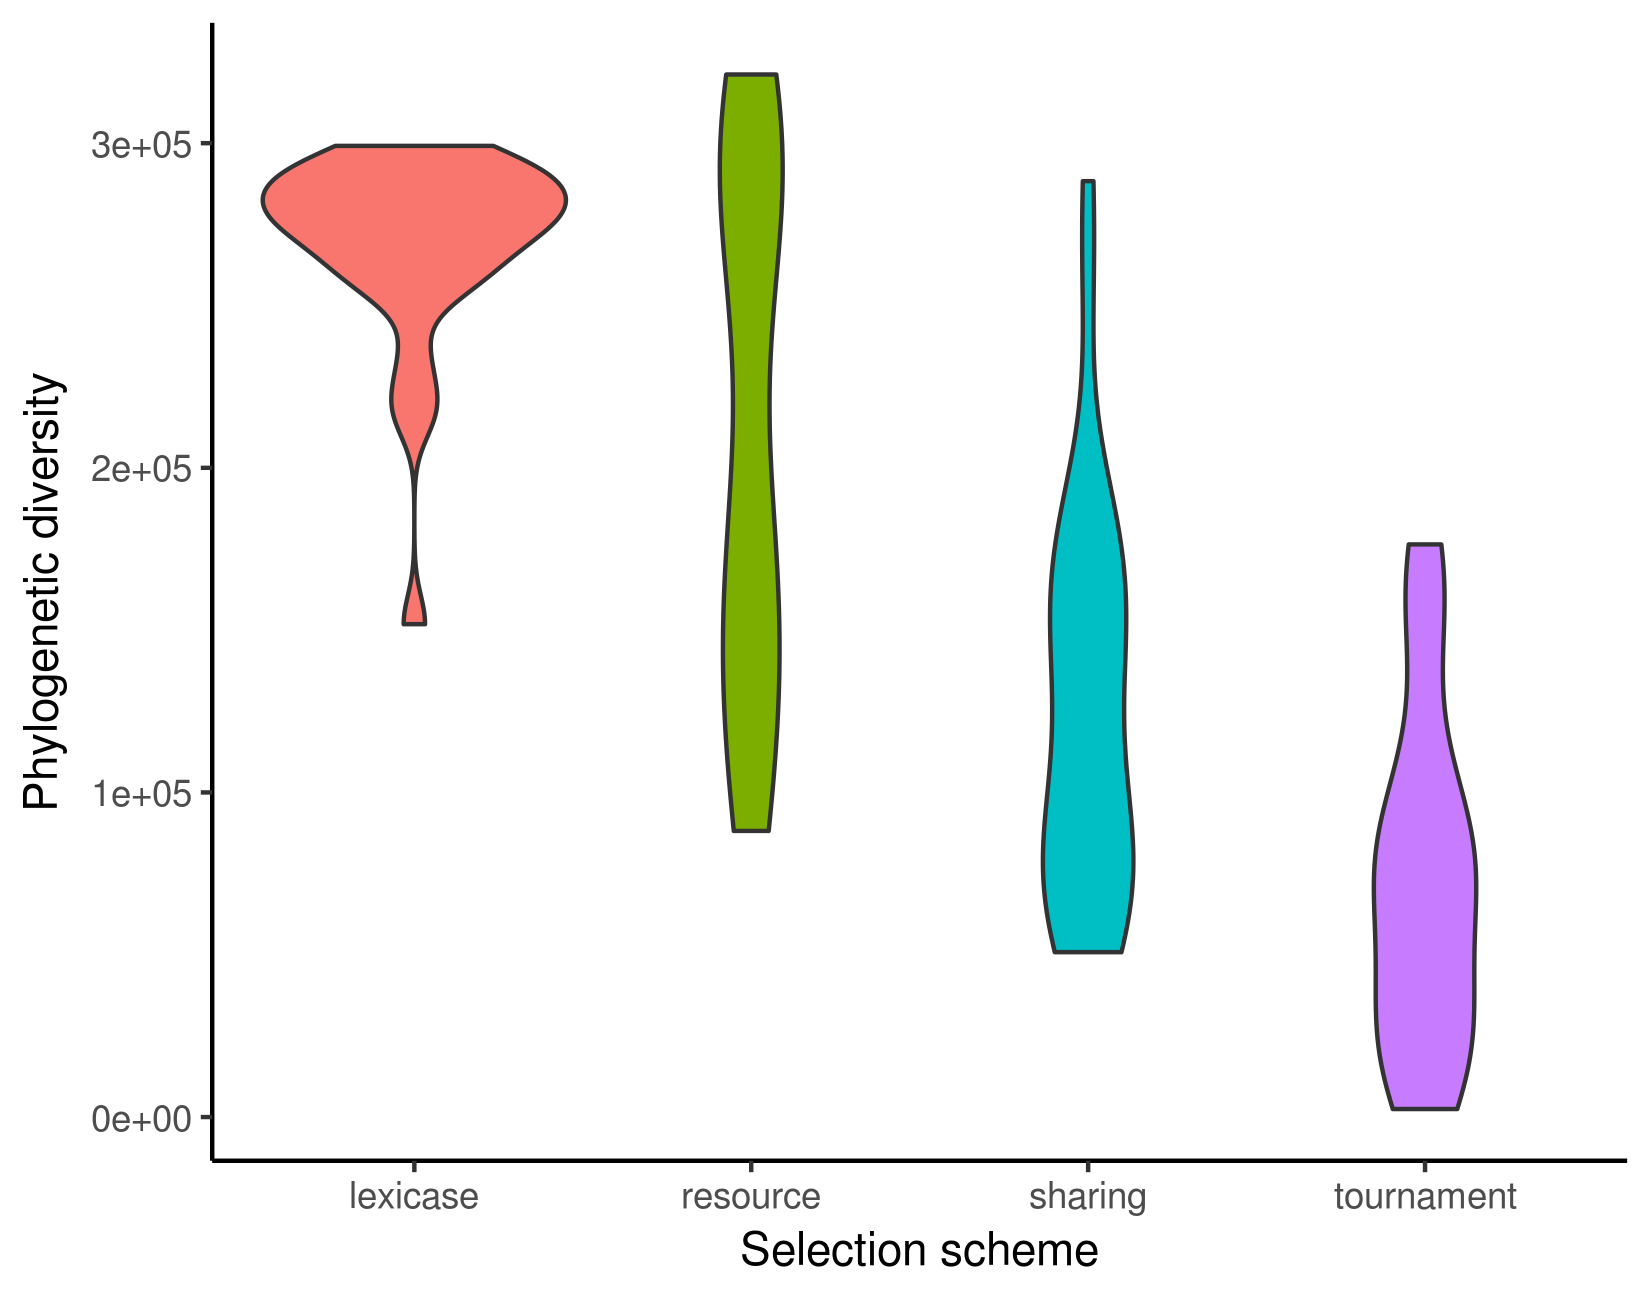
\includegraphics[width=1.6in]{figs/phylo_all.png}
%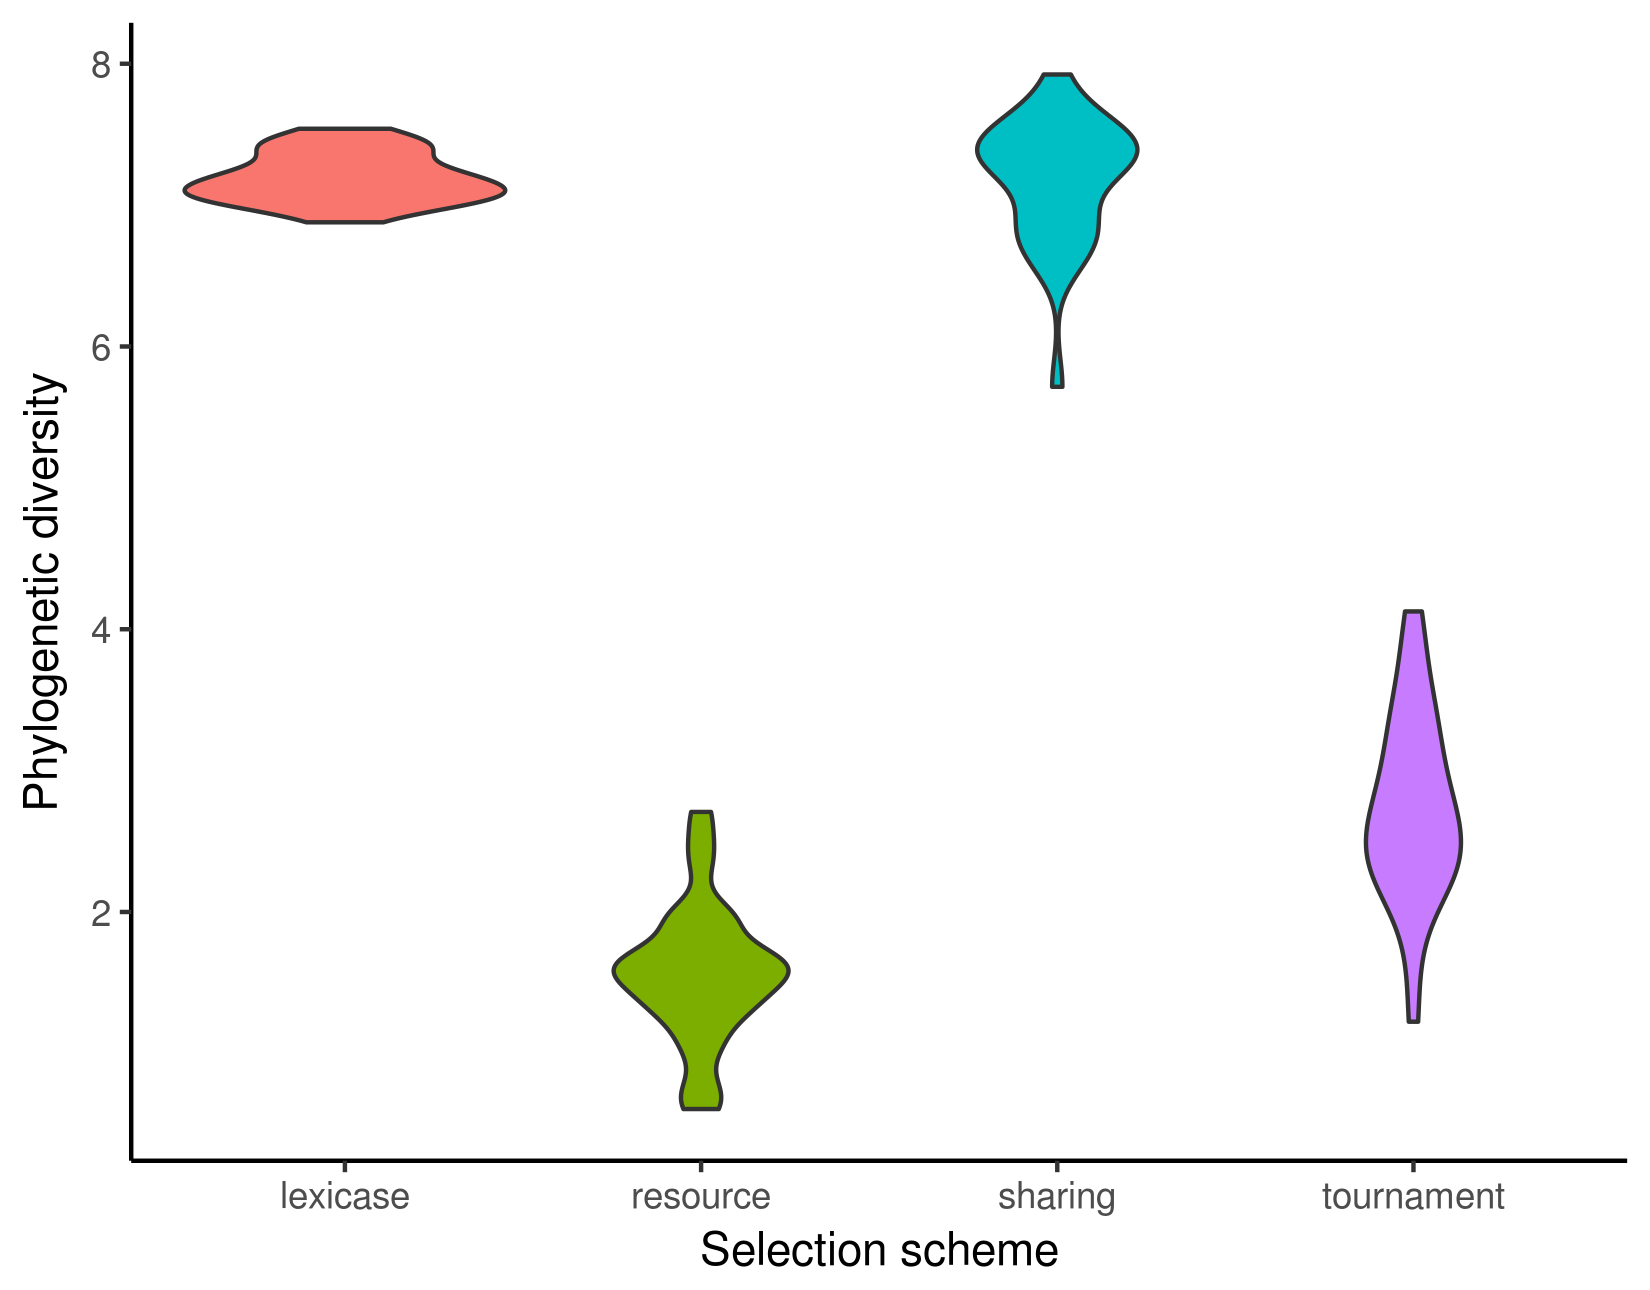
\includegraphics[width=1.6in]{figs/pheno_all.png}
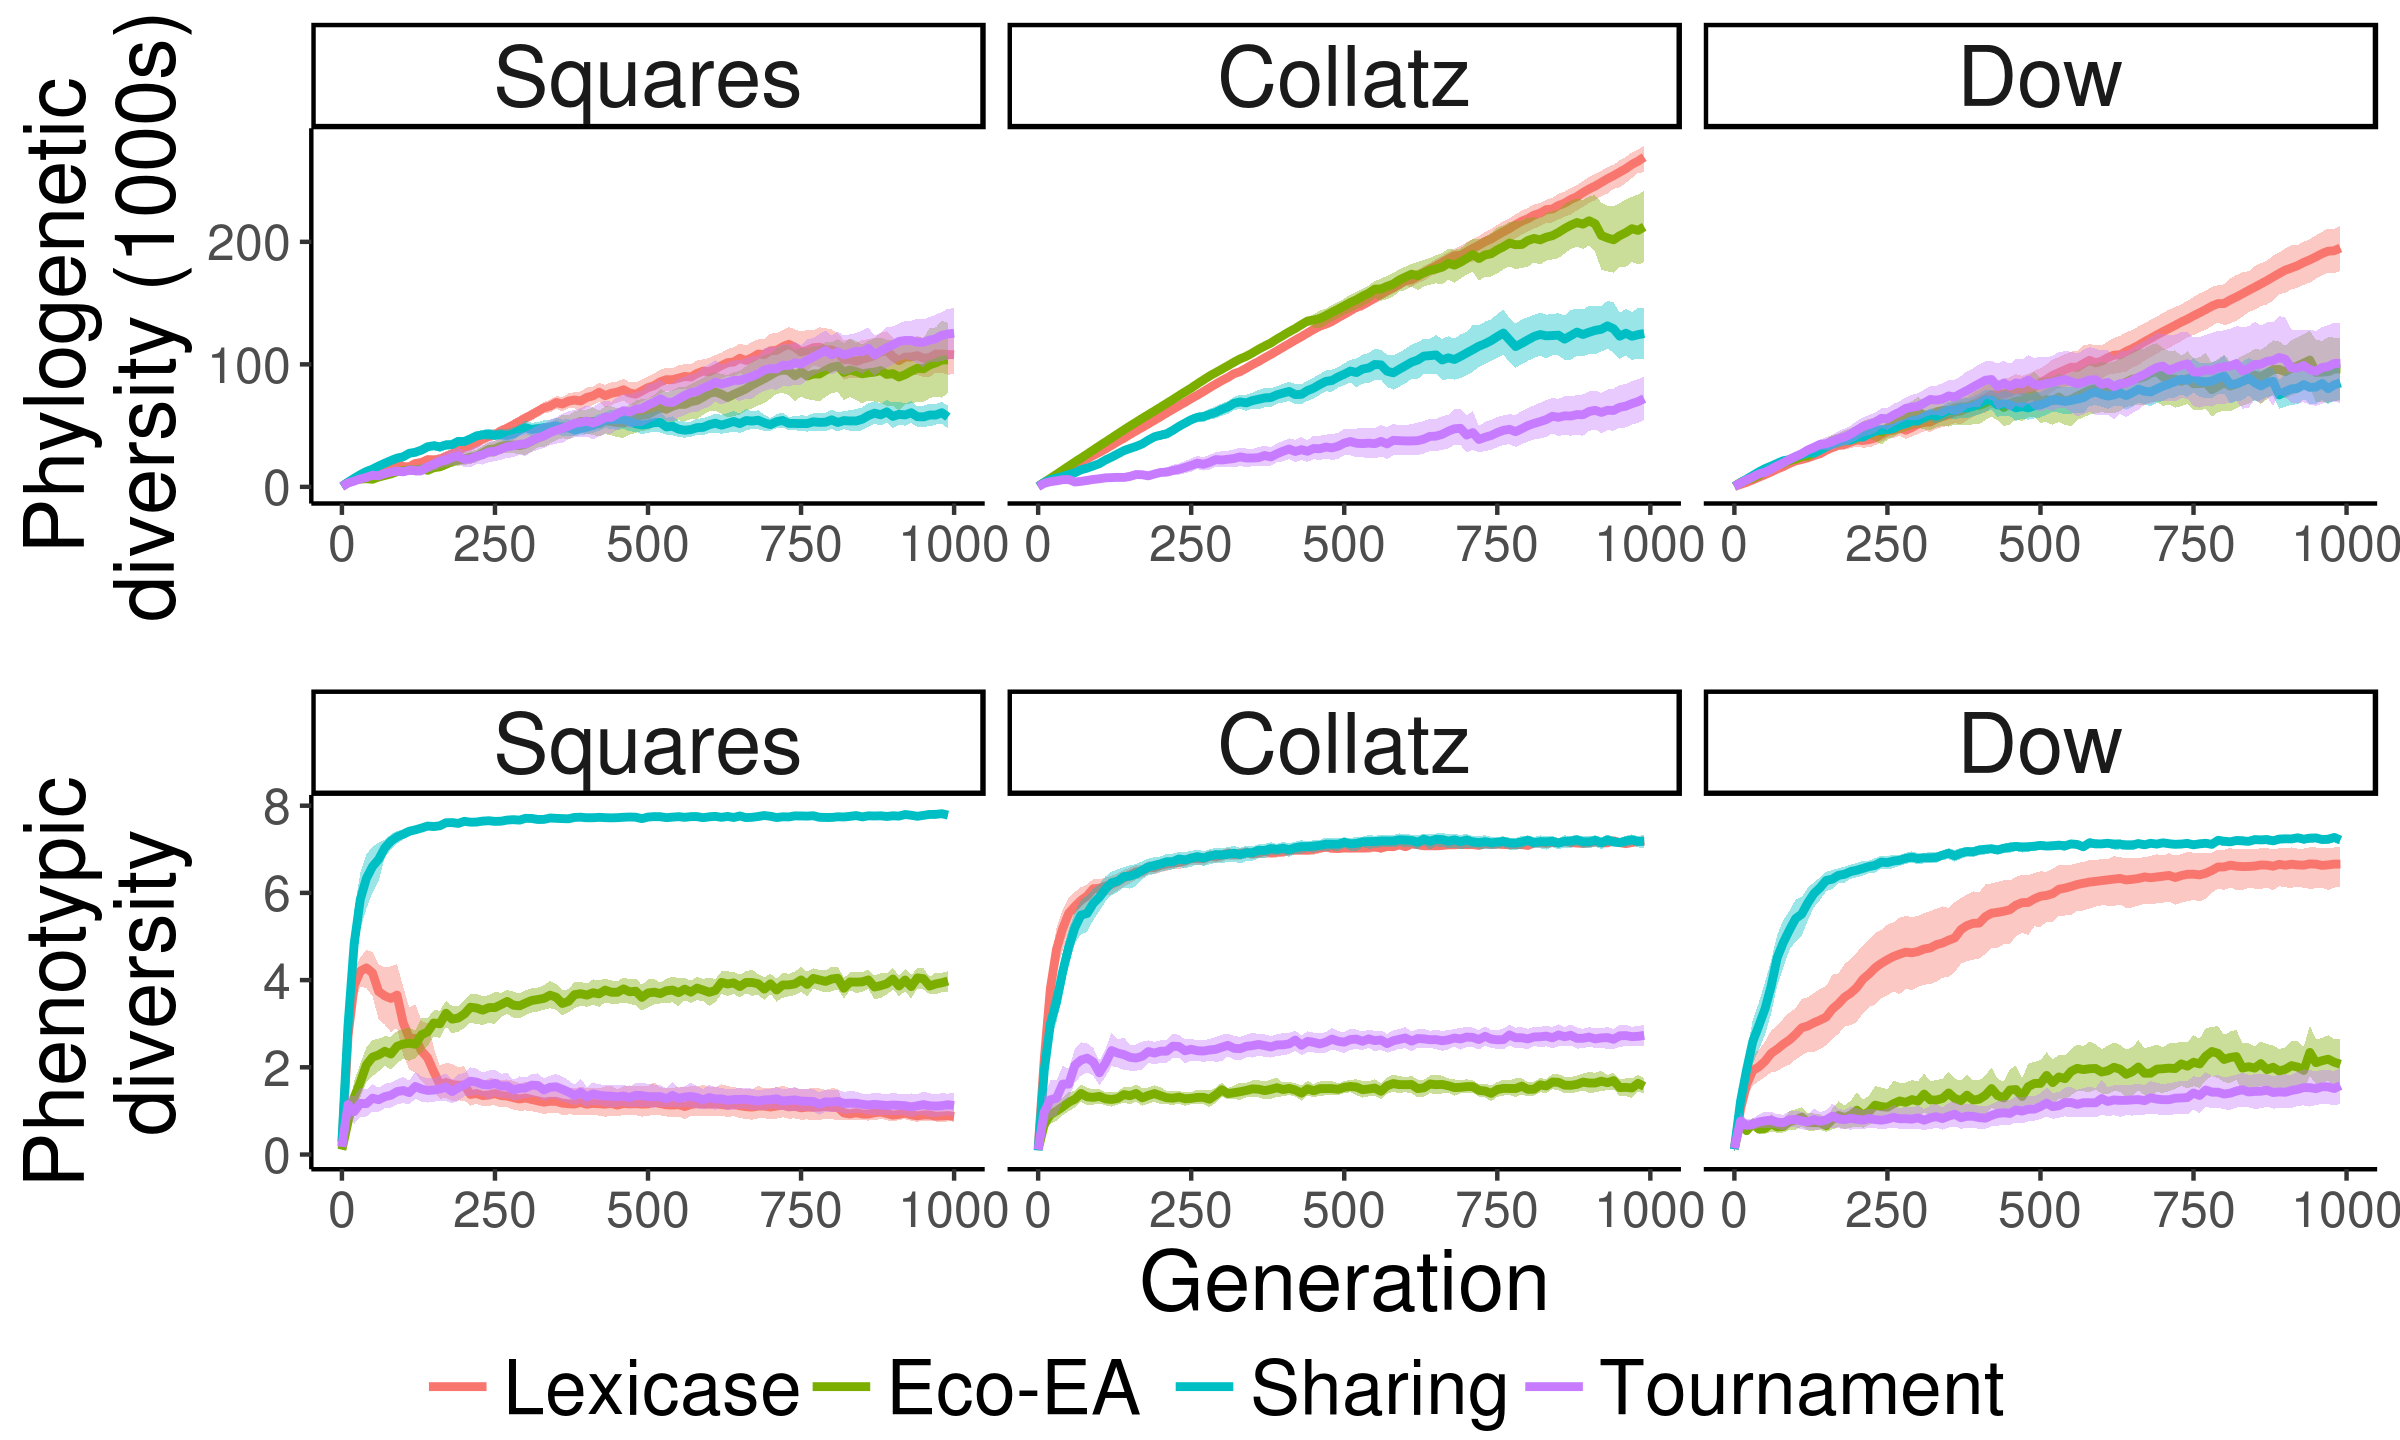
\includegraphics[width=3.4in]{figs/time_all.png}
\caption{Phentypic and phylogenetic diversity over time for each problem. Shaded area is the bootstrapped 95\% confidence interval around the mean.}
\label{phylo_results}
\end{figure}

As hypothesized, phylogenetic diversity is low for all selection schemes on the square problem (see Figure \ref{phylo_results}). This result is presumably due to fitness differences so large that stabilizing effects are insufficient to overcome them. In the context of such a steep evolutionary gradient, such behavior is expected and often desirable. Due to negative frequency dependence, phenotypic diversity remains high for fitness sharing and Eco-EA, even after most populations solved the problem (generally between 200 and 500 generations in). %This may also be related to the fact that there are many solutions to the squares problem.
For lexicase selection, on the other hand, it initially increases and then drops rapidly as the populations converge on the solution.

Results from the Collatz problem support our hypothesis that selection schemes with more restrictions on which individuals compete %with which others
promote phylogenetic diversity (see Figure \ref{phylo_results}). Lexicase selection and Eco-EA did not have significantly different final phylogenetic diversity (Wilcoxon rank-sum test, p=0.31), but all other pairs of selection schemes did (Wilcoxon rank-sum tests, p $<$ .05). Results for mean pairwise distance were similar, suggesting that lexicase selection and Eco-EA (and to a lesser extent fitness sharing) do promote the coexistence of divergent branches. 

Interestingly, phenotypic diversity does not correlate especially closely with phylogenetic diversity (see Figure \ref{phylo_results}). In particular, Eco-EA has relatively low phenotypic diversity, despite its high phylogenetic diversity. Conversely, fitness sharing has relatively high phenotypic diversity despite its mid-range phylogenetic diversity. This result suggests that whereas lexicase selection and fitness sharing allow similar phenotypes to coexist, Eco-EA forces them to converge. A potential explanation for this difference is that Eco-EA rewards generalists substantially more than lexicase selection.

\begin{figure}
%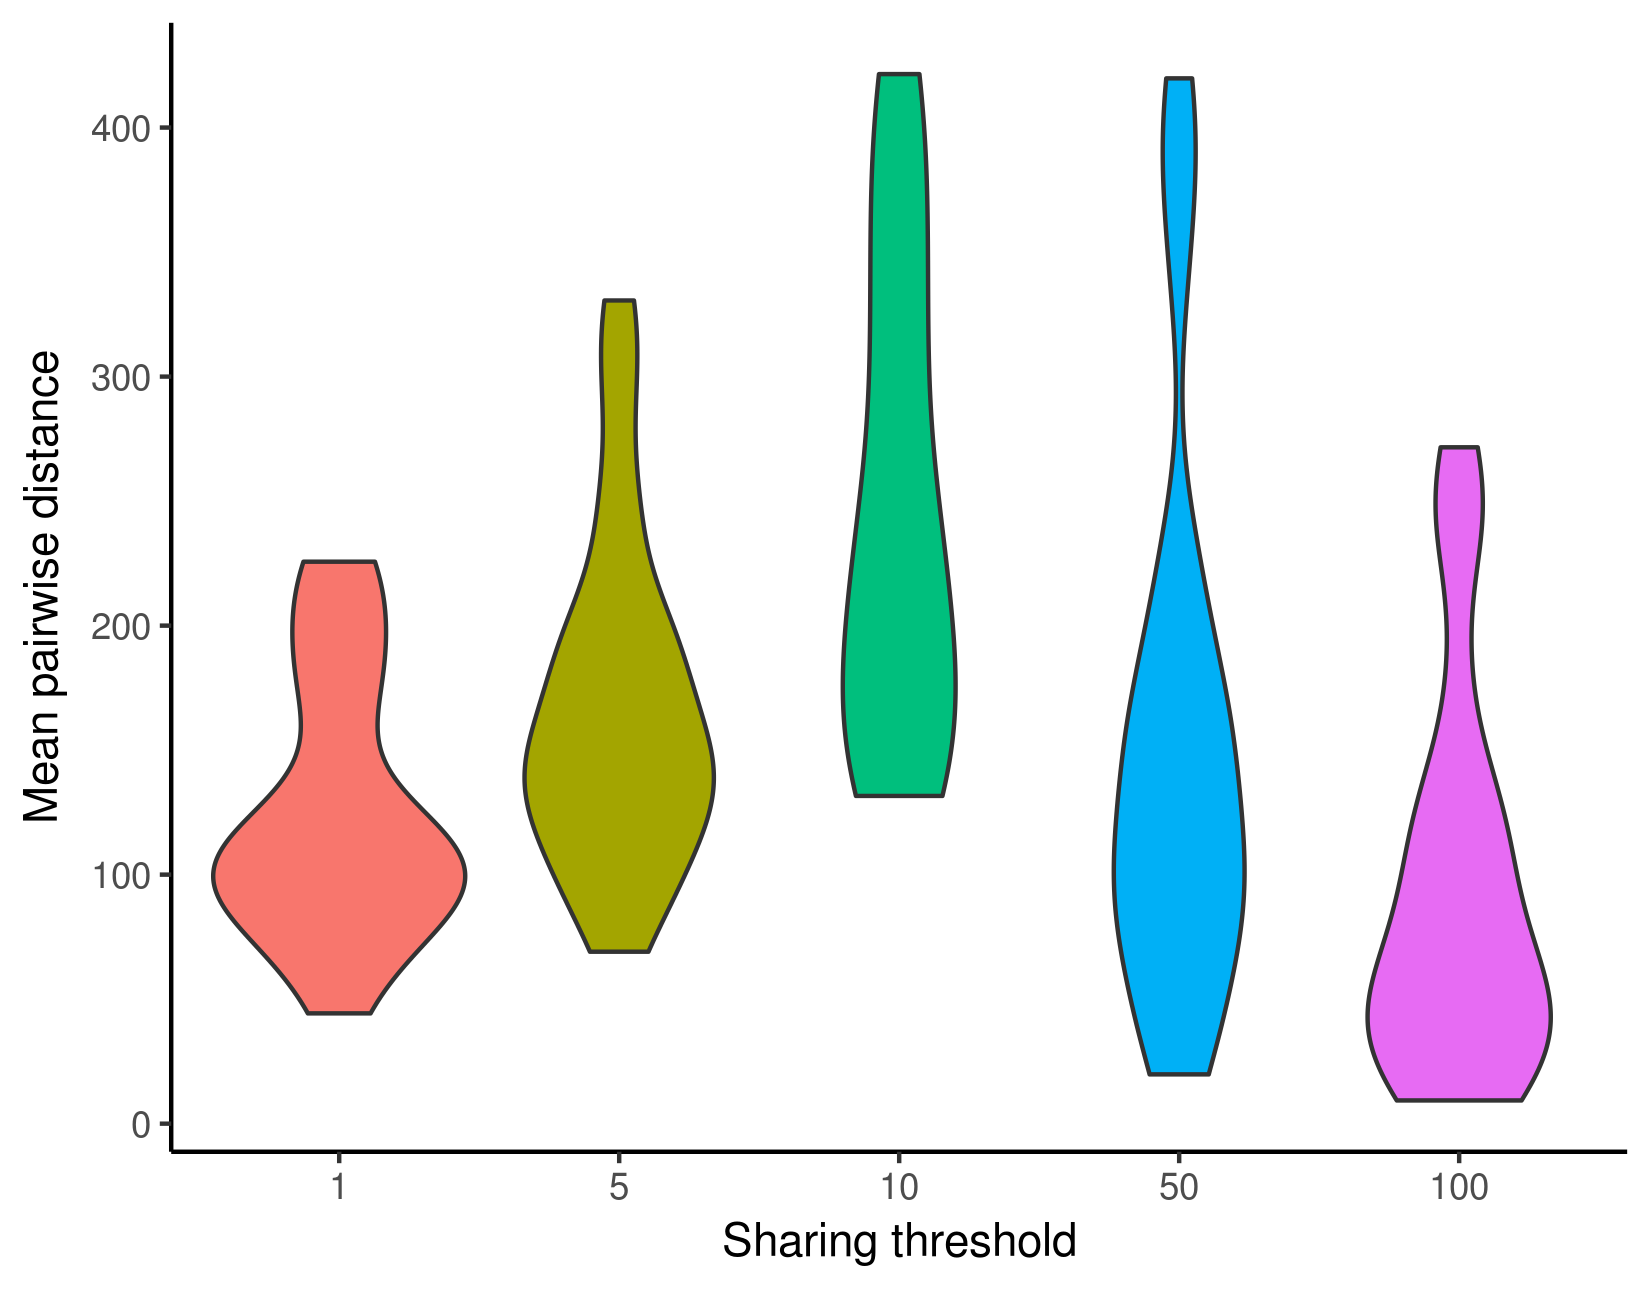
\includegraphics[width=1.6in]{figs/sharing_pairwise_dist.png}
%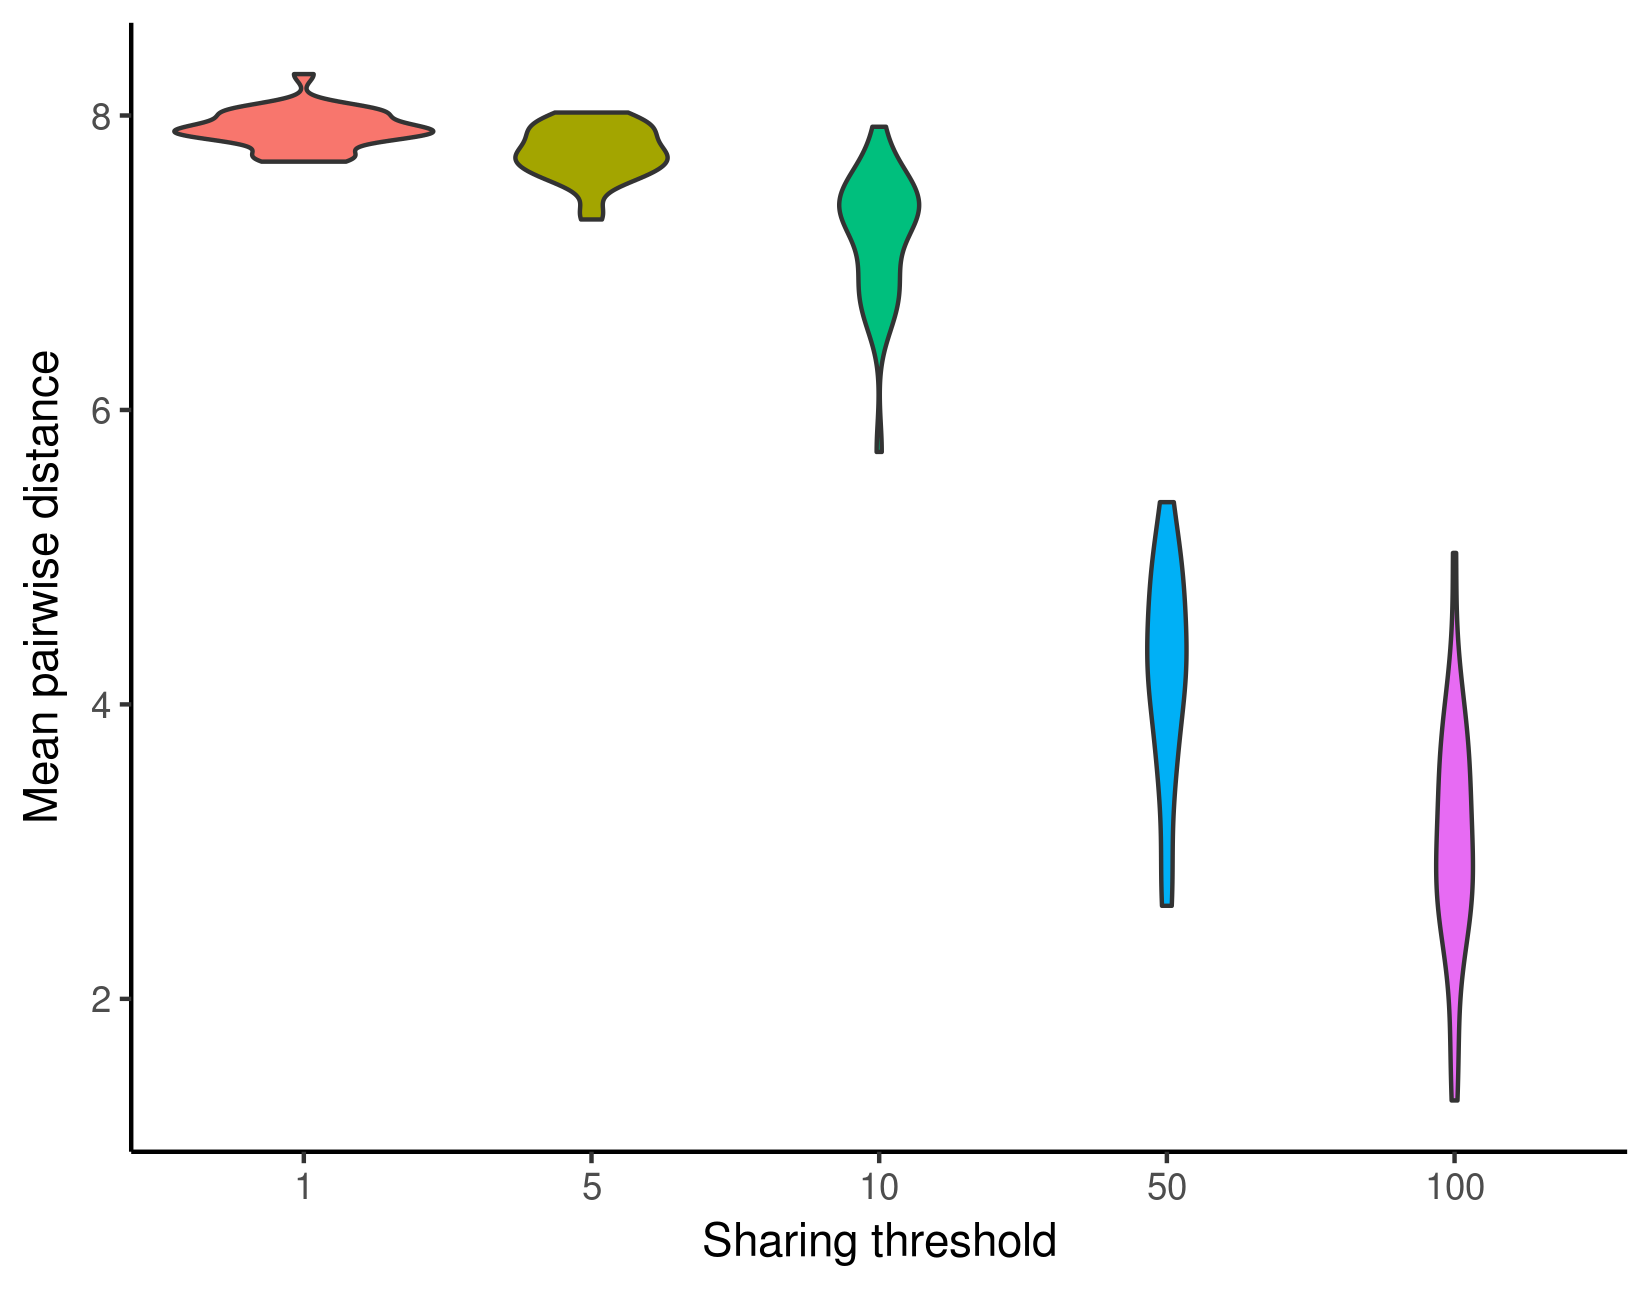
\includegraphics[width=1.6in]{figs/sharing_phenotypic_entropy.png}
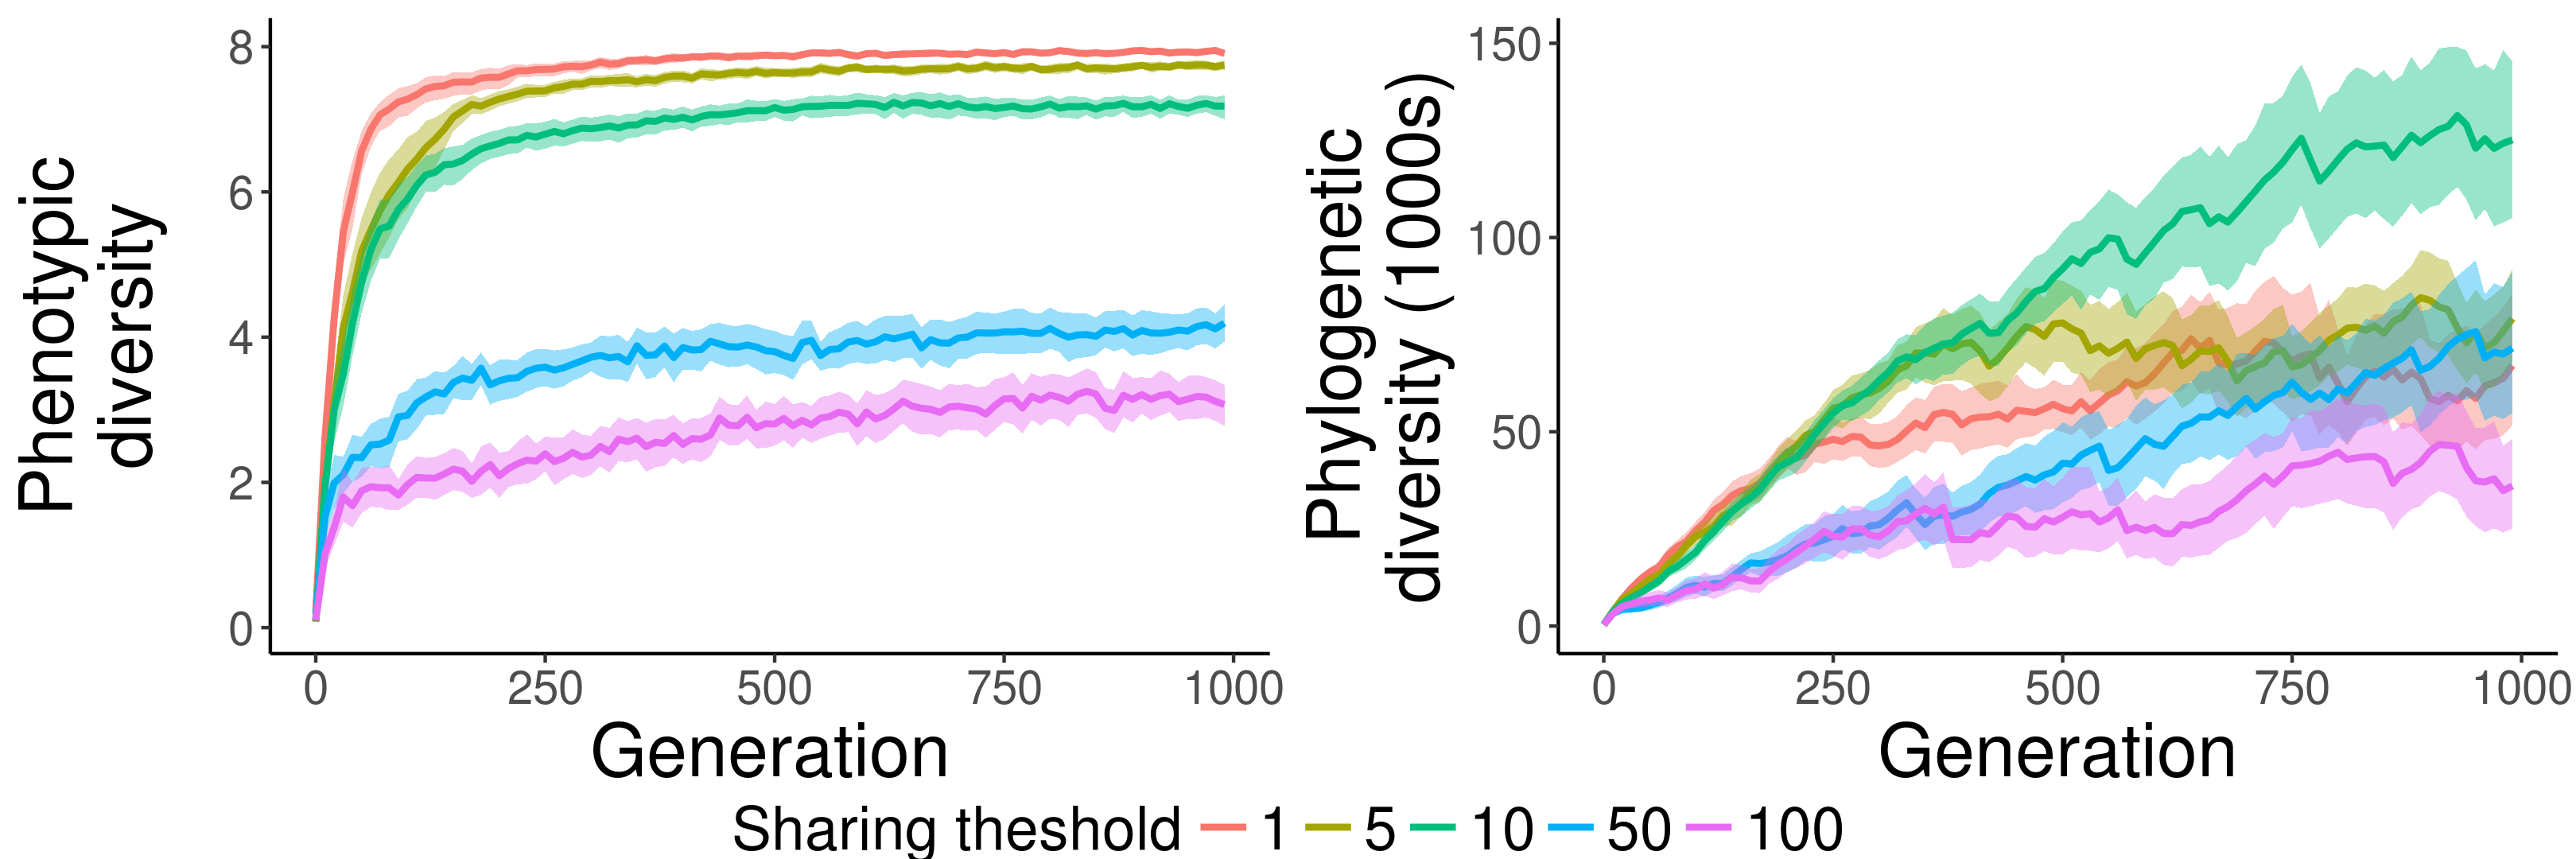
\includegraphics[width=3.4in]{figs/time_sharing.png}
\caption{Phenotypic and phylogenetic diversities across various values of sharing threshold ($\sigma_{\text{share}}$) in the context of the Collatz problem. Shaded area is the bootstrapped 95\% confidence interval around the mean.}
\label{sharing}
\end{figure}

This discrepancy is even more pronounced in the context of selecting a sharing threshold for fitness sharing (see Figure \ref{sharing}). Phenotypic diversity is maximized at  $\sigma_{\text{share}} = 1$  (Wilcoxon rank-sum tests, p $<$ .005), whereas mean pairwise distance and phylogenetic diversity are highest at $\sigma_{\text{share}} = 10$  (Wilcoxon rank-sum tests, p $<$ .005). This result emphasizes the fact that phylogenetic diversity is meaningfully different from phenotypic and genotypic diversity in ways that can affect choice of parameter values.

Results from the Dow problem (see Figure \ref{phylo_results}) illustrate the strong effect that the topology of the fitness landscape has on which techniques are most effective at maintaining phylogenetic diversity. In contrast to its high efficacy on the Collatz problem, Eco-EA maintains no more phylogenetic diversity than fitness sharing and tournament selection on the Dow chemical problem (Wilcoxon rank-sum tests, p = 1 for all). Lexicase selection, on the other hand, maintains phylogenetic diversity on both of these problems (Wilcoxon rank-sum tests, p $<$ .005). Understanding what properties of the fitness landscape account for this difference is an important area of future research.

\section{Conclusions}

In this paper, we have taken a high-level tour of tools that ecology can contribute to EC. Using metaphors and mathematical theory from ecology, we have identified
important differences across four selection schemes. Importantly, we have shown mathematical equivalence between rules governing coexistence in ecology and in EC. This framework should allow us to directly translate insights between these fields.

Building on this conceptual understanding, we empirically measured the interactions that describe the communities created by different selection schemes. The topology of these interaction networks supports our theoretical predictions, and provides insight into the mechanisms by which these techniques maintain diversity. A more systematic study of interaction networks under various selection schemes will further improve our understanding. We gained further insight by exploring the long-term effects of these selection schemes with phylogenetic metrics. Notably, we demonstrated that phylogenetic analysis metrics describe aspects of the underlying dynamics of diversification that are distinct from those described by genotypic and phenotypic diversity. This result holds across different parameter choices for the same selection scheme, and across different selection schemes. Analyzing the phylogenies of populations evolving on a wider range of fitness landscapes has the potential to help predict which parameters and selection schemes are most appropriate for which problems.

From our analysis thus far, we can conclude that lexicase selection and Eco-EA use distinct underlying mechanisms to promote the evolution and maintenance of solutions that are evolutionarily divergent. Lexicase selection creates a small number of intense competitive interactions, whereas Eco-EA creates a larger number of weaker interactions that can be either competitive or facilitative. As a result, lexicase selection generates %a large number of
many specialist phenotypes, while Eco-EA supports
%a smaller number of 
fewer, more generalist phenotypes. Phenotypes from both selection schemes are more evolutionarily distinct than those evolved under fitness sharing, and are expected to fall somewhere along the Pareto front.

Ecological techniques have the power to revolutionize our understanding of diversity in EC, and our work here has barely %scratched the surface
started. In the future, we plan to delve deeper into these approaches, to import more ideas and statistical techniques from ecology, and to apply them to an even wider range of selection schemes.

\begin{acks}
Removed for anonymous review.
%We thank Alex Lalejini, Matthew Moreno, and Michael Wiser for their helpful comments and suggestions on early drafts of this manuscript. This research has been supported by the National Science Foundation (NSF) BEACON Center under Cooperative Agreement DBI-0939454, by an NSF Graduate Research Fellowship to ED under Grant No. DGE-1424871, and by Michigan State University through computational resources provided by the Institute for Cyber-Enabled Research. Any opinions, findings, and conclusions or recommendations expressed in this material are those of the author(s) and do not necessarily reflect the views of the NSF.
\end{acks}


% \subsection{Citations}
% Citations to articles~\cite{bowman:reasoning,
% clark:pct, braams:babel, herlihy:methodology},
% conference proceedings~\cite{clark:pct} or maybe
% books \cite{Lamport:LaTeX, salas:calculus} listed
% in the Bibliography section of your
% article will occur throughout the text of your article.
% You should use BibTeX to automatically produce this bibliography;
% you simply need to insert one of several citation commands with
% a key of the item cited in the proper location in
% the \texttt{.tex} file~\cite{Lamport:LaTeX}.
% The key is a short reference you invent to uniquely
% identify each work; in this sample document, the key is
% the first author's surname and a
% word from the title.  This identifying key is included
% with each item in the \texttt{.bib} file for your article.

% The details of the construction of the \texttt{.bib} file
% are beyond the scope of this sample document, but more
% information can be found in the \textit{Author's Guide},
% and exhaustive details in the \textit{\LaTeX\ User's
% Guide} by Lamport~\shortcite{Lamport:LaTeX}.

% This article shows only the plainest form
% of the citation command, using \texttt{{\char'134}cite}.

% Some examples.  A paginated journal article \cite{Abril07}, an enumerated
% journal article \cite{Cohen07}, a reference to an entire issue \cite{JCohen96},
% a monograph (whole book) \cite{Kosiur01}, a monograph/whole book in a series (see 2a in spec. document)
% \cite{Harel79}, a divisible-book such as an anthology or compilation \cite{Editor00}
% followed by the same example, however we only output the series if the volume number is given
% \cite{Editor00a} (so Editor00a's series should NOT be present since it has no vol. no.),
% a chapter in a divisible book \cite{Spector90}, a chapter in a divisible book
% in a series \cite{Douglass98}, a multi-volume work as book \cite{Knuth97},
% an article in a proceedings (of a conference, symposium, workshop for example)
% (paginated proceedings article) \cite{Andler79}, a proceedings article
% with all possible elements \cite{Smith10}, an example of an enumerated
% proceedings article \cite{VanGundy07},
% an informally published work \cite{Harel78}, a doctoral dissertation \cite{Clarkson85},
% a master's thesis: \cite{anisi03}, an online document / world wide web
% resource \cite{Thornburg01, Ablamowicz07, Poker06}, a video game (Case 1) \cite{Obama08} and (Case 2) \cite{Novak03}
% and \cite{Lee05} and (Case 3) a patent \cite{JoeScientist001},
% work accepted for publication \cite{rous08}, 'YYYYb'-test for prolific author
% \cite{SaeediMEJ10} and \cite{SaeediJETC10}. Other cites might contain
% 'duplicate' DOI and URLs (some SIAM articles) \cite{Kirschmer:2010:AEI:1958016.1958018}.
% Boris / Barbara Beeton: multi-volume works as books
% \cite{MR781536} and \cite{MR781537}.

% A couple of citations with DOIs: \cite{2004:ITE:1009386.1010128,
%   Kirschmer:2010:AEI:1958016.1958018}. 

% Online citations: \cite{TUGInstmem, Thornburg01, CTANacmart}.  


% \subsection{Tables}
% Because tables cannot be split across pages, the best
% placement for them is typically the top of the page
% nearest their initial cite.  To
% ensure this proper ``floating'' placement of tables, use the
% environment \textbf{table} to enclose the table's contents and
% the table caption.  The contents of the table itself must go
% in the \textbf{tabular} environment, to
% be aligned properly in rows and columns, with the desired
% horizontal and vertical rules.  Again, detailed instructions
% on \textbf{tabular} material
% are found in the \textit{\LaTeX\ User's Guide}.

% Immediately following this sentence is the point at which
% Table~\ref{tab:freq} is included in the input file; compare the
% placement of the table here with the table in the printed
% output of this document.

% \begin{table}
%   \caption{Frequency of Special Characters}
%   \label{tab:freq}
%   \begin{tabular}{ccl}
%     \toprule
%     Non-English or Math&Frequency&Comments\\
%     \midrule
%     \O & 1 in 1,000& For Swedish names\\
%     $\pi$ & 1 in 5& Common in math\\
%     \$ & 4 in 5 & Used in business\\
%     $\Psi^2_1$ & 1 in 40,000& Unexplained usage\\
%   \bottomrule
% \end{tabular}
% \end{table}

% To set a wider table, which takes up the whole width of the page's
% live area, use the environment \textbf{table*} to enclose the table's
% contents and the table caption.  As with a single-column table, this
% wide table will ``float'' to a location deemed more desirable.
% Immediately following this sentence is the point at which
% Table~\ref{tab:commands} is included in the input file; again, it is
% instructive to compare the placement of the table here with the table
% in the printed output of this document.


% \begin{table*}
%   \caption{Some Typical Commands}
%   \label{tab:commands}
%   \begin{tabular}{ccl}
%     \toprule
%     Command &A Number & Comments\\
%     \midrule
%     \texttt{{\char'134}author} & 100& Author \\
%     \texttt{{\char'134}table}& 300 & For tables\\
%     \texttt{{\char'134}table*}& 400& For wider tables\\
%     \bottomrule
%   \end{tabular}
% \end{table*}
% % end the environment with {table*}, NOTE not {table}!

% It is strongly recommended to use the package booktabs~\cite{Fear05}
% and follow its main principles of typography with respect to tables:
% \begin{enumerate}
% \item Never, ever use vertical rules.
% \item Never use double rules.
% \end{enumerate}
% It is also a good idea not to overuse horizontal rules.


% \subsection{Figures}

% Like tables, figures cannot be split across pages; the best placement
% for them is typically the top or the bottom of the page nearest their
% initial cite.  To ensure this proper ``floating'' placement of
% figures, use the environment \textbf{figure} to enclose the figure and
% its caption.

% This sample document contains examples of \texttt{.eps} files to be
% displayable with \LaTeX.  If you work with pdf\LaTeX, use files in the
% \texttt{.pdf} format.  Note that most modern \TeX\ systems will convert
% \texttt{.eps} to \texttt{.pdf} for you on the fly.  More details on
% each of these are found in the \textit{Author's Guide}.

% %\begin{figure}
% %
\includegraphics{fly}
% %\caption{A sample black and white graphic.}
% %\end{figure}

% %\begin{figure}
% %
\includegraphics[height=1in, width=1in]{fly}
% %\caption{A sample black and white graphic
% %that has been resized with the \texttt{includegraphics} command.}
% %\end{figure}


% As was the case with tables, you may want a figure that spans two
% columns.  To do this, and still to ensure proper ``floating''
% placement of tables, use the environment \textbf{figure*} to enclose
% the figure and its caption.  And don't forget to end the environment
% with \textbf{figure*}, not \textbf{figure}!

% %\begin{figure*}
% %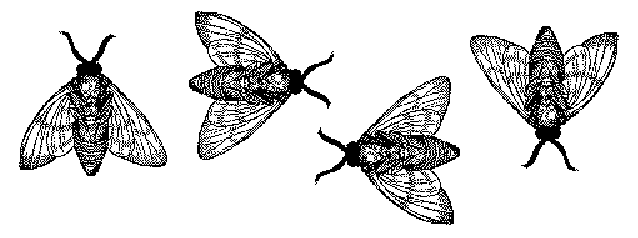
\includegraphics{flies}
% %\caption{A sample black and white graphic
% %that needs to span two columns of text.}
% %\end{figure*}


% %\begin{figure}
% %
\includegraphics[height=1in, width=1in]{rosette}
% %\caption{A sample black and white graphic that has
% %been resized with the \texttt{includegraphics} command.}
% %\end{figure}

% \subsection{Theorem-like Constructs}

% Other common constructs that may occur in your article are the forms
% for logical constructs like theorems, axioms, corollaries and proofs.
% ACM uses two types of these constructs:  theorem-like and
% definition-like.

% Here is a theorem:
% \begin{theorem}
%   Let $W$ be continuous on $[a,b]$.  If $G$ is
%   an antiderivative for $W$ on $[a,b]$, then
%   \begin{displaymath}
%     \int^b_af(t)\,dt = G(b) - G(a).
%   \end{displaymath}
% \end{theorem}

% Here is a definition:
% \begin{definition}
%   If $z$ is irrational, then by $e^z$ we mean the
%   unique number that has
%   logarithm $z$:
%   \begin{displaymath}
%     \log e^z = z.
%   \end{displaymath}
% \end{definition}

% The pre-defined theorem-like constructs are \textbf{theorem},
% \textbf{conjecture}, \textbf{proposition}, \textbf{lemma} and
% \textbf{corollary}.  The pre-defined de\-fi\-ni\-ti\-on-like constructs are
% \textbf{example} and \textbf{definition}.  You can add your own
% constructs using the \textsl{amsthm} interface~\cite{Amsthm15}.  The
% styles used in the \verb|\theoremstyle| command are \textbf{acmplain}
% and \textbf{acmdefinition}.

% Another construct is \textbf{proof}, for example,

% \begin{proof}
%   Suppose on the contrary there exists a real number $L$ such that
%   \begin{displaymath}
%     \lim_{x\rightarrow\infty} \frac{f(x)}{g(x)} = L.
%   \end{displaymath}
%   Then
%   \begin{displaymath}
%     l=\lim_{x\rightarrow c} f(x)
%     = \lim_{x\rightarrow c}
%     \left[ g{x} \cdot \frac{f(x)}{g(x)} \right ]
%     = \lim_{x\rightarrow c} g(x) \cdot \lim_{x\rightarrow c}
%     \frac{f(x)}{g(x)} = 0\cdot L = 0,
%   \end{displaymath}
%   which contradicts our assumption that $l\neq 0$.
% \end{proof}

% \section{Conclusions}
% This paragraph will end the body of this sample document.
% Remember that you might still have Acknowledgments or
% Appendices; brief samples of these
% follow.  There is still the Bibliography to deal with; and
% we will make a disclaimer about that here: with the exception
% of the reference to the \LaTeX\ book, the citations in
% this paper are to articles which have nothing to
% do with the present subject and are used as
% examples only.
% %\end{document}  % This is where a 'short' article might terminate



% \appendix
% %Appendix A
% \section{Headings in Appendices}
% The rules about hierarchical headings discussed above for
% the body of the article are different in the appendices.
% In the \textbf{appendix} environment, the command
% \textbf{section} is used to
% indicate the start of each Appendix, with alphabetic order
% designation (i.e., the first is A, the second B, etc.) and
% a title (if you include one).  So, if you need
% hierarchical structure
% \textit{within} an Appendix, start with \textbf{subsection} as the
% highest level. Here is an outline of the body of this
% document in Appendix-appropriate form:
% \subsection{Introduction}
% \subsection{The Body of the Paper}
% \subsubsection{Type Changes and  Special Characters}
% \subsubsection{Math Equations}
% \paragraph{Inline (In-text) Equations}
% \paragraph{Display Equations}
% \subsubsection{Citations}
% \subsubsection{Tables}
% \subsubsection{Figures}
% \subsubsection{Theorem-like Constructs}
% \subsubsection*{A Caveat for the \TeX\ Expert}
% \subsection{Conclusions}
% \subsection{References}
% Generated by bibtex from your \texttt{.bib} file.  Run latex,
% then bibtex, then latex twice (to resolve references)
% to create the \texttt{.bbl} file.  Insert that \texttt{.bbl}
% file into the \texttt{.tex} source file and comment out
% the command \texttt{{\char'134}thebibliography}.
% % This next section command marks the start of
% % Appendix B, and does not continue the present hierarchy
% \section{More Help for the Hardy}

% Of course, reading the source code is always useful.  The file
% \path{acmart.pdf} contains both the user guide and the commented
% code.

